%%%%%%%%%%%%%%%%%%%%%%%%%%%%%%%%%%%%
% This is the template for submission to ISCA 2018
% The cls file is a modified from  'sig-alternate.cls'
%%%%%%%%%%%%%%%%%%%%%%%%%%%%%%%%%%%%

\documentclass{sig-alternate} 
\usepackage{mathptmx} % This is Times font

\newcommand{\ignore}[1]{}
\usepackage{fancyhdr}
\usepackage[normalem]{ulem}
\usepackage[hyphens]{url}
\usepackage{microtype}
\usepackage{fixltx2e}
\usepackage{array}
\usepackage{multirow}
\usepackage{graphicx}
\usepackage{changepage}
\usepackage{color}
\usepackage{flushend}
\usepackage{adjustbox}
\usepackage{setspace}
\graphicspath{ {./graphs/}{./figures/} }
\newcommand{\pg}[1]{{{\color{blue}PG: {#1}}}}

% Always include hyperref last
\usepackage[bookmarks=true,breaklinks=true,letterpaper=true,colorlinks,linkcolor=black,citecolor=blue,urlcolor=black]{hyperref}

% Ensure letter paper
\pdfpagewidth=8.5in
\pdfpageheight=11in


%%%%%%%%%%%---SETME-----%%%%%%%%%%%%%
\newcommand{\iscasubmissionnumber}{34}
%%%%%%%%%%%%%%%%%%%%%%%%%%%%%%%%%%%%

\fancypagestyle{firstpage}{
  \fancyhf{}
\renewcommand{\headrulewidth}{0pt}
  \fancyhead[C]{\normalsize{}} 
  \fancyfoot[C]{\thepage}
}  

\pagenumbering{arabic}
\fancypagestyle{firstpage}{
  \fancyhf{}
\renewcommand{\headrulewidth}{0pt}
  \fancyhead[C]{\normalsize{ISCA 2019 Submission
      \textbf{\#\iscasubmissionnumber} \\ Confidential Draft: DO NOT DISTRIBUTE}}
  \fancyfoot[C]{\thepage}
}

%%%%%%%%%%%---SETME-----%%%%%%%%%%%%%
\title{Perceptron-Based Prefetch Filtering} 
\author{}
%%%%%%%%%%%%%%%%%%%%%%%%%%%%%%%%%%%%

\begin{document}
\maketitle
\thispagestyle{firstpage}
\pagestyle{plain}

\begin{spacing}{0.99}
\begin{abstract}
Hardware prefetching has been introduced in modern processors as a way to hide
cache latencies.  An efficient prefetcher should be able to identify complex
memory access patterns during program execution. This ability enables the
prefetcher to read a block ahead of its demand access, potentially saving a
cache miss. Accurately identifying the right blocks to prefetch is essential
to achieving high performance from the prefetcher.

In this paper, we introduce Perceptron-based Prefetch Filtering to help make
this prefetching decision accurately. The perceptron layer acts as a check 
to filter out the unnecessary prefetches recommended by the underlying
prefetcher.  We have also explored a range of features that can be used to
train the perceptron layer.  Our results show that perceptron-based filtering
improves performance on the memory intensive subset of the SPEC 2017 benchmark
suite by 6.84\% on single-core and by 11.9\% on multi-core traces, as compared
to a state-of-the art prefetcher.  We also demonstrate that the performance
gained from using our efficient filter scales better with increasing numbers
of cores.

\end{abstract}

\section{Introduction}
\label{Introduction}

Processor and memory technologies have been developed with different
goals in mind. While processor scaling has focused on speed
improvements, memory scaling has primarily focused on increasing
capacity. The difference in each technology's scaling has led to the
Memory Wall~\cite{MemWall} -- the increasing gap between processor and
memory performance. Data prefetching is one important technique that
has been developed to minimize the effects of this trend.

%Data prefetching exploits the fact that in most applications,
% memory accesses have a repeating and predictable pattern to speculatively fetch useful data from slower levels
%of the cache hierarchy into faster higher levels of cache. %phrasing?

An ideal prefetching scheme would perfectly capture a program's memory
access pattern, and then predict and pre-load the needed data into the
processor's caches in a timely manner.  Memory access patterns may be
simple, such as accessing every item in an array with a for-loop, or
very complex, such as chasing pointers through dynamically-allocated
memory.  % Practical prefetchers face challenges not only in predicting
% what data will be useful in the future, but also in timing when data
% should be prefetched, deciding which level of the cache hierarchy the
% data should be stored in, and deciding what data should be evicted
% from the caches to accommodate the prefetched data.
All prefetchers are designed around a fundamental trade-off between
two important metrics: coverage and accuracy. Prefetcher coverage
refers to the fraction of baseline cache misses that the prefetcher
pulls into the cache prior to their reference.  For example, if an
application experiences 1,000 cache misses without a prefetcher, while
800 of those cache misses become hits with a prefetcher, then the
prefetcher has 80\% coverage for that application.  Prefetcher
accuracy refers to the fraction of prefetched cache lines that end up
being used by the application. So if a prefetcher prefetches 1,200
cache lines, but only 800 of them are used by the application, then
that prefetcher's accuracy is 66.7\%.


\begin{figure}[t]
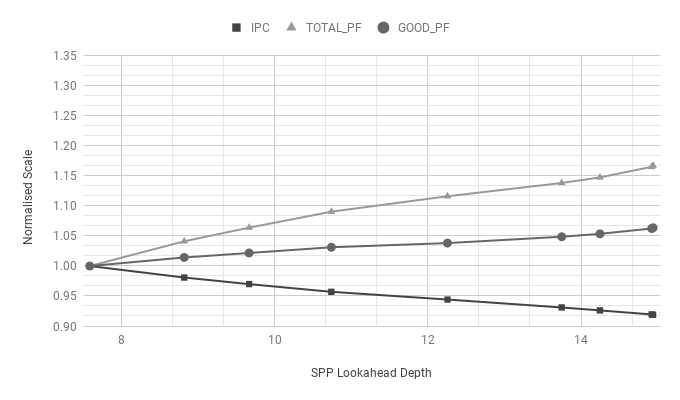
\includegraphics[width=\columnwidth]{Motivation}
\caption{The impact of aggressive prefetching on performance for {\tt 603.bwaves\_s}. 
The number of useful prefetches increases with aggressiveness
slower than total prefetches, which wastes bandwidth and 
harms performance.}
\label{Fig:Motivation}
\end{figure}

Coverage and accuracy are generally at odds with one another, and as
one metric improves, the other usually gets worse. For example, when
an application accesses a new region of memory for the first time, a
na\"ive prefetcher may predict that all data in that region will be
used by the application.  This will clearly result in 100\% coverage
for that region, but with possibly a very low accuracy.  In fact, so
much cache capacity and bandwidth may be wasted prefetching unused
data that performance can ultimately be harmed by this strategy. At
the other extreme, another prefetcher may be overly conservative and
never prefetch anything, wasting no capacity or bandwidth, and
achieving 0\% prefetch coverage.

Figure~\ref{Fig:Motivation} illustrates the above scenario.  Here we
consider a state-of-the-art lookahead prefetcher -- SPP~\cite{SPP}.
Lookahead prefetchers such as SPP provide a mechanism to speculate an
arbitrary number of references ahead of the initial triggering miss.
In SPP, a throttling confidence threshold is then used to ensure that
the lookahead stops when confidence falls too low to ensure that
prefetches are accurate.  In the figure, we iteratively re-tuned 
this threshold to allow the prefetcher to lookahead a fixed
depth from 7 to 15. The figure depicts the behavior 
of the {\tt 603.bwaves\_s} SPEC CPU 2017 benchmark. The IPC, the 
total number of prefetches issued by the prefetcher (TOTAL\_PF), 
and the actual useful predictions (GOOD\_PF), all have been normalized 
to lookahead depth 7. As the lookahead
depth increases, so do useful prefetches, and hence coverage. This
coverage, however, comes at the cost of total prefetches increasing at
an even higher rate. This leads to cache pollution and bandwidth
contention, and leads to a reduction in IPC.  
%Similar behavior was observed in 12 other SPEC CPU 2017 benchmarks.

Therefore, a delicate balance between coverage and accuracy is
required for a prefetcher to maximize its performance impact.
Prefetchers are generally designed with internal mechanisms to monitor
their accuracy, and throttling mechanisms that can be tuned for either
coverage or accuracy.  The more irregular an application's memory
access pattern is, the more difficult it is to accurately predict
every access, so a prefetcher will have to be tuned more toward
coverage (and away from accuracy) in order to gain any benefit. This
may be especially dangerous to do in the context of a multi-core
processor, where overly aggressive prefetching in one core can waste
shared resources, such as last-level cache (LLC) capacity, and
off-chip bandwidth, impacting the performance of other
cores~\cite{Friendly}.

% Predicting future accesses requires a trade-off between coverage,
% the percent of predictions that prevented a cache miss, and
% accuracy, the percent of predictions made that were correct.
%% Gino: Just added a short explanation of coverage and accuracy
%% tradeoff, not sure if necessary
%A prefetcher may have high coverage by reducing the number of misses
% by simply requesting a large amount of data, however this does not
% imply accuracy. Even if the prefetcher brought in data accessed in
% the future, a high percentage of the data requested could never be
% accessed meaning the prefetcher had low accuracy, resulting in
% wasted resources as well as cache pollution. Likewise, a prefetcher
% can have a higher accuracy by being completely sure the data
% requested is used in the future, but may not affect performance
% since it did not have the coverage needed to make an
% impact. %end addition.
% Most prefetchers maintain an internal confidence mechanism by
% keeping counters to track events such as cache hits, misses,
% references to an entry in the prefetcher's structure, etc. By
% comparing the confidence indicated by the counters against different
% threshold values, the aggressiveness of the prefetcher can be
% adjusted, resulting in lower coverage and higher accuracy.

%For a prefetcher to capture highly irregular access patterns, it
% needs to be highly aggressive with high coverage. This causes the
% prefetcher to recommend many low accuracy prefetches that lead to
% the cache being polluted with useless data.  This effect is more
% pronounced in a multi-core scenario where the LLC is a shared
% resource~\cite{Friendly}. Conversely, a conservative prefetcher
% would be highly accurate but might not make enough useful prefetches
% due to its lower coverage.

Here, we propose Perceptron-based Prefetch Filtering (PPF) as an
enhancement to existing state-of-the-art prefetchers, allowing them to
speculate deeply to achieve high coverage while filtering out the
inaccurate prefetches this deep speculation implies.  PPF works by
observing the stream of candidate prefetches generated by a
prefetcher, and then rejects those that are predicted by the
online-trained neural model to be inaccurate.  The state-of-the-art
prefetcher that we use to evaluate PPF in this paper is the Signature
Path Prefetcher (SPP)~\cite{SPP}, however as we describe, PPF can be
designed to benefit any prefetcher.  In this design, PPF replaces
SPP's existing confidence-based throttling mechanism, which itself was
a highly tuned feature of that prefetcher.  Because PPF is so much
more effective at rejecting inaccurate prefetches than SPP's 
{\color{red}internal} mechanism, we are free to re-tune the rest of 
SPP's design around maximizing coverage. The result is an increase 
in both accuracy and coverage, and a notable increase in performance.

%We propose Perceptron-based Prefetch Filtering (PPF) as an enhancement to
%the existing state of the art prefetchers to robustly overcome the coverage
%vs. accuracy trade-off. The idea is to use a state-of-the-art prefetcher as
%the base engine. For that we choose Signature Path Prefetcher (SPP) and
%modify the design to make it as aggressive as possible. This modification
%enables the base engine to capture complex memory access patterns and go
%deeper into the speculation path, increasing coverage without sacrificing accuracy. 
%Normally such aggressive prefetching would come at the cost of increased DRAM traffic
%and cache pollution. However, prefetch suggestions recommended by the base prefetch
%engine are passed through the perceptron based filter to ensure an accurate prediction.
%Over time, PPF learns to correlate the prefetch recommendations with various available
%features, leading to elimination of useless prefetches. This filtering leads
%to overall increased accuracy of the prefetch scheme and reduction in DRAM
%traffic and cache pollution.

This paper describes PPF, explains its merits, offers analysis, and
outlines the scope for future research. Its contributions are:

\begin{itemize}

\item An on-line neural model used for hardware data prefetching.
  Previous work in this area either relied on program
  semantics~\cite{Semantics} or were application
  specific~\cite{Datacenter}.

\item Implementing PPF filtering a state-of-the-art prefetcher, giving
  a significant performance improvement compared to previous work. PPF
  learns to adapt itself to shared resource constraints, leading to
  further increased performance in multi-core and
  bandwidth-constrained environments.

\item A methodology for determining an appropriate set of features for
  prediction, regardless of the underlying prefetcher used.  More
  details are explained in Section \ref{Method-Features}.

\end{itemize}

In a single core configuration, PPF increases performance by 3.78\%
compared to the underlying prefetcher, SPP. In a multi-core system running a
mixes of memory intensive SPEC CPU 2017 traces, PPF saw an improvement
of 11.4\% over SPP for a 4-core system, and 9.65\% for an 8-core system.

% djimenez - cutting this
%The paper is organized as follows. Section~\ref{Background} describes
%background work and summarizes SPP. Section~\ref{Arch} gives the 
%architectural overview of PPF. Section~\ref{Impl} discusses the
%implementation of PPF using SPP and the particular features used.
%Section~\ref{Method} gives the evaluation methodology and explores the feature
%space for perceptron learning. Section~\ref{Results} evaluates the
%performance of the prefetcher and Section~\ref{Conclusion} concludes the
%paper.

\section{Background Work and Motivation}
\label{Background}

In this section, we compare the existing work done in the domain of
prefetching.  We also discuss about some of the interesting memory
access patterns seen in the workloads in SPEC 2017 benchmark.  The
second half of this section deals with a background of Signature Path
Prefetcher architecture.

\subsection{Related Work}
\label{Background-Related}
The idea of prefetching has been around since Instruction Stream
Buffers were proposed by Jouppi~\cite{ISB}. Some of the earliest data
prefetchers developed to try to identify memory access patterns with a
constant stride pattern~\cite{Smith,Baer,Stride}. Major research was
dedicated to stride distance and depth prediction~\cite{Decoupled,Adaptive}. Newer prefetchers aimed at correlating
predictions with the past memory access addresses~\cite{Address_Correlated,AMPM}.

With time newer and more intricate prefetchers were
introduced~\cite{Wenisch_Temporal_Streaming,Stealth,Feedback_Directed,Coordinated,Bandwidth_Efficient,Pacman,TLB,Linearizing,Sandbox,VLDP,DoL,Domino}.
A whole class of streaming prefetchers developed on the lines of
Spatial / Temporal Memory
Streaming~\cite{Spatial_Pattern,SMS,Temporal_Instruction_Fetch,Off_Chip,STMS,SMS_JILP}.
There have been ideas for control flow speculation directed hardware prefetching~\cite{BFetch,MTBFetch}.

Most modern prefetchers aim at identifying complex memory access
patterns in a given application.  This allows them to capture some of
the irregular patterns seen in pointer chasing data-structures.
Offset based prefetchers are a generalization of the next-line
prefetcher.  Some of the prominent prefetchers exploiting this idea
are Sandbox Prefetcher~\cite{Sandbox} and the Best Offset Prefetcher~\cite{BOP}. 
Another class of prefetchers is lookahead Prefetchers.
Such prefetchers try to speculate deep into the application's memory
access trail.  These include Path Confidence based Lookahead
Prefetching~\cite{SPP} and Kill the Program Counter~\cite{KPC}.

A related line of work also explores cache replacement - insertion
policies and dead block prediction, with an eye towards
prefetching~\cite{DB_Pred,Cache_Burst,KPC,Harmony}.  Nori
\textit{et.al.} introduced prefetching with respect to runtime
criticality~\cite{CATCH}.

\textit{Machine Learning and Prefetching:} Peled \textit{et.al.}
introduce interesting ideas for on-line Reinforcement Learning and
dynamically scaling the magnitude of feedback given to the baseline
prefetcher~\cite{Semantics}. The biggest challenge here is that it
relies on compiler support for getting features to build the context.

The paper by Liao \textit{et. al.} focuses on prefetching for data
center applications~\cite{Datacenter}. They use offline Machine
Learning Algorithms like SVMs and Logistic Regressions to do
parametric search for an optimal prefetcher configuration.

%% NOTE: The below paper is literally the same idea as ours. But poor implementation and no good results. How much to bash this paper?
Finally, the paper on Data Cache Prefetching with Perceptron
Learning~\cite{BadPerc} talks about the idea of two step prefetching.
The first step is an existing baseline prefetcher while the second
step is a perceptron based throttler.  The paper has lots of
limitations in terms of design and implementation.  That reflects in
the fact that it did not lead to any significant performance gain over
even the basic prefetchers like the Stride Prefetcher~\cite{Stride} and
the Markov Prefetcher~\cite{Markov}.


\subsection{Perceptron Learning in Architecture}
\label{Background-Perceptron}
Perceptron learning for computer architecture design has been around
for a while.  It was first popularized by Jimenez \textit{et. al.} for
doing branch prediction~\cite{Perc_Branch}. In it's original
implementation, the Program Counter of the instruction looking for a
branch prediction would index into a given table of perceptron
weights.  The retrieved weights would then be multiplied with the
history of branch outcomes stored in the History Register (which is a
feature) in a dot product fashion.  The sum obtained is thresholded at
0 \textit{i.e.}, if the prediction y\textsubscript{out} >= 0, the
prediction is made as \textit{true}, or branch taken.  Else if the sum
is < 0, the prediction is made as \textit{false}.

The structure that we use is derived from the model introduced in
Piecewise Linear Branch Prediction~\cite{Piece_Linear}.  Here the
feature itself is used to index into a hash of perceptron weights.
This form of indexing makes sure that the hyper-plane learned by the
perceptron weights is able to differentiate between linearly
inseparable outcomes.  \textit{<Is it true? Not sure>}

Perceptron Learning for Reuse Prediction~\cite{Perc_Reuse} extended the
hash perceptron architecture to perform prediction in context of cache
replacement.  Perceptron layer can learn to correlate the cache
replacement behaviour with a variety of features.  Each feature has
its dedicated table of perceptron weights which it indexes into.
Hence number of tables equals the number of features.  Once the
perceptron weights from all the tables are obtained, they're summed
and thresholded based on a pre-decided value.  This led to a
prediction mechanism that is highly accurate, has quick learning rate
and is adaptable to changing program behaviour.  The features
introduced in that paper were derived from Program Counters of the
current and the last few instructions and from the memory address of the
current access.  Even with such basic features, high level of
correlation could be established by perceptrons.

The work was further extended by Multiperspective Reuse
Prediction~\cite{Multiperspective}, which introduced a varied set of
parametric features.  Although design space exploration for feature
and parameter selection was a non-trivial task, once fixed, it could
give a cache replacement predictor highly suitable for the given set
of applications.

\textit{Deviations From Actual Perceptrons:} Traditionally, a
perceptron prediction involves multiplying the vector of input
features: F\textsubscript{1xN}, with the corresponding weight vector:
W\textsubscript{Nx1} in a dot product fashion to obtain the sum
y\textsubscript{out}.  Here what we use is a perceptron-like
structure.  The feature is used to hash into the weight of perceptrons
and the retrieved weights are added straight away.  This can be seen a
dot product of $\vec{1}$\textsubscript{1xN} with W\textsubscript{Nx1}.
This way, the perceptron algorithm doesn't introduce any
multiplication operations in the inference or training process.  Hence
what we adapt in this work, is a perceptron-like learning algorithm as
it involves the same principle involved in perceptron inferencing and
training.  For simplicity, we will call our implementation as
perceptron implementation.

\textit{Perceptron Update Rule:} In all the above implementations, a
uniform perceptron update principle is being followed.  The weights
need to be updated if the prediction was wrong or the predicted sum
does not cross a certain threshold.  After a certain training period,
these weights are proportional to the probability of the outcome being
true.  This training threshold makes sure that the perceptrons are
trained till a certain level of confidence and yet they are not
over-trained to the given set.  Care is taken that the weights
saturate at certain positive and negative values so that they remain
confined to the bit-width.  The same rules will be applied in the
discussion done in Section \ref{Design-Perceptron} on NATCH learning algorithm.

 
\subsection{Prefetching with SPEC 2017}
\label{Background-SPEC2017}
\textit{<Discuss SPEC 2017 traces here>
<What are the possible graphs / analysis tools we can use for SPEC traces?>}

\subsection{Signature Path Prefetcher Architecture}
\label{Background-SPP}
Since the work we have done uses SPP~\cite{SPP} as the underlying prefetcher, we are
presenting a brief recap of the ideas introduced in the original
paper, especially with an eye towards their relevance in our work.
Signature Path Prefetcher (SPP) is a lookahead prefetcher and consists
of following structural components:

\textbf{Signature Table:} The ST keeps track of 256 most recently accessed
pages.  It is meant to capture memory access patterns within a page
boundary.  SPP indexes into an entry of ST using the page number.  For
each entry corresponding to a page, ST stores the `last block offset'
and `old signature'.  Last block offset is the block offset of the
last memory access of that given page.  The block offset is calculated
with respect to the page boundary.  The signature is a 12-bit
compressed representation of the past few memory accesses for that
page.  The signature is calculated as:
$$New Signature = (\,Old Signature << 3 bits\,) \;\;XOR\;\; (\,Delta\,)$$ 
In case a matching page entry is found, the stored signature in the corresponding entry is retrieved.

%% NOTE: Can we do away with this example? 
%%       If it looks like we are weiting too much about SPP
Consider the case that incoming page number 10 with a block offset 3
finds a match in the ST.  The retrieved pattern signature is 0x30 and
the Last Offset is 1.  Since now there is the Last Block Offset (1),
Incoming Block Offset (3), Old Signature (0x30), and New Signature
calculated as per above equation (0x182), SPP can infer
non-speculatively that the given pattern of memory accesses (as
captured in the Old Signature) leads to the particular Delta.  In
general, Delta is defined as the difference between the prefetch
suggestion block and the initial block which triggered the prefetch.
In this case, since SPP is in learning phase, it is defined as the
difference between the Incoming Block Offset and the Last Block Offset
(+2 in this case).  This, in turn generates the new memory pattern
(New Signature).  This newly learned signature pattern and the delta
is stored in the Pattern Table.

\textbf{Pattern Table:} The PT is indexed by the signature generated
from ST.  PT holds predicted delta patterns and their confidence
estimates.  Each entry indexed by the signature holds up to 4 unique
delta predictions.  This is implemented by making PT as a 4-way
associative table.  To measure an estimate of a delta confidence, PT
implements two counters: C\textsubscript{sig} for each entry indexed
by the signature and C\textsubscript{delta} for each delta entry for a
given signature.  More details of this on-line score-keeping mechanism
is described under Confidence Tracking discussion.

\textit{Lookahead Prefetching:} On each trigger, SPP tries to go down
the program speculation path using its own prefetch suggestion.
Using current prefetch as the baseline, it re-accesses the PT to generate further
prefetches.  It keeps on repeating this cycle of accessing PT and
updating the signature based on highest confidence prefetch from the
last iteration.  These iteration count till which SPP manages to
predict prefetch entries in the lookahead manner is characterized as
its `depth'.  While doing this, SPP also keeps compounding the
confidence in each depth.  Thus as depth increases, overall confidence
keeps decreasing.  

\textbf{Global History Register:} The GHR is a small 8-entry fully
associative structure to bootstrap learning across page boundaries. 
Whenever a prefetch suggestion from the
Pattern Table crosses page boundaries, instead of completely
discarding it, GHR saves that information for inter-page learning.
Since our NATCH implementation in this paper doesn't affect GHR
functionality in any ways, we won't be going into more details about
GHR.

\textbf{Prefetch Filter:} SPP also introduced the concept of Prefetch
Filter - a 1024 entry 1-way associative table which keeps a record of
last few entries prefetched.  This proves useful for following
reasons:
\begin{itemize}
\item \textbf{Eliminating duplicate prefetches}\newline Any subsequent
  prefetches recommended by SPP mechanism are checked against the
  existing entries in Prefetch Filter.  If a valid entry is found, it
  means that the particular cache line is already either in L2 Cache
  or being fetched.  Hence there is no need to issue a duplicate
  prefetch.
    
\item \textbf{Updating prefetcher}\newline Since the PF keeps a track
of past few prefetches, it uses that information to see if a given
prefetch led to a demand hit or a cache eviction. Using this information, 
SPP can update its internal states.
    
\item \textbf{Tracking Global Accuracy}\newline PF keeps a track of
  global usefulness ($\alpha$) of the prefetches by calculating 
  C\textsubscript{useful} / C\textsubscript{total}, where
  C\textsubscript{total} is the total number of prefetches
  getting recorded in the PF and C\textsubscript{useful} is the number 
  of prefetches that led to a demand hit.
\end{itemize}

\textbf{Confidence Tracking}: The PT keeps a track of hits to each
signature through a counter C\textsubscript{sig}.  The number of hits
for a given delta per signature are tracked using a counter
C\textsubscript{delta}.  The confidence for a given delta is
approximated through C\textsubscript{d} = C\textsubscript{delta} /
C\textsubscript{sig}.  When SPP enters into a lookahead mode, the path
confidence P\textsubscript{d} is given as:
$$P\textsubscript{d} \;=\; \alpha  \;.\;  C\textsubscript{d}  \;.\;  P\textsubscript{d-1}$$ where $\alpha$ is called the global accuracy and is calculated as shown previously. 
The range of global accuracy ($\alpha$) is [0,1].

Here d is the lookahead depth.  For d = 1, when SPP is in
non-speculative mode, P\textsubscript{0} can be thought of as 1. 
The final P\textsubscript{d} is thresholded against prefetching-threshold
(T\textsubscript{p}) to decide whether to prefetch or not.  If yes,
then P\textsubscript{d} is thresholded against a numerically bigger
fill-threshold (T\textsubscript{f}) to decide whether the prefetch
should be sent to L2 Cache (high confidence prefetch) or Last Level
Cache (low confidence prefetch)

<Insert a comprehensive figure about SPP structures>

<Insert another detailed picture about SPP data-path flow>

\subsection{Case for an On-line Throttler}
\label{Background-Case}
As compared to some of the other state of the art prefetchers [BOP],
SPP is a less aggressive prefetcher.  In the single core
environment, this gives BOP an edge as there is no resource contention
among the different cores.  Hence more aggressive prefetching is bound
to prove beneficial.  As we increase the core count, we observe that
SPP starts outperforming rest of the prefetchers.  This can be
attributed to the fact that each prefetch suggested by SPP is a
carefully calculated one and that prevents cache pollution.
\textit{<Figure showing the variation of SPP vs BOP wrt core count>}
For 4-core applications, SPP suggests XX\% fewer prefetches than BOP
and yet leads to higher IPC.

The above analysis shows that with a more careful throttling
mechanism, any prefetcher like SPP can be tuned to become much more aggressive, leading to
increased coverage.  The onus of maintaining the accuracy now falls on
the independent throttler.  To test the hypothesis, we tuned down SPP
to the minimum possible threshold.  Only by doing this we managed to
increase the prefetch suggestions made by SPP, by XX\%.
\textit{<Comparison of SPP-Unleased with SPP / BOP>} Obviously this
came at a cost of increased DRAM traffic and cache pollution.

Moreover, the on-line confidence mechanism introduced in SPP was very
rudimentary.  It was based on taking a ratio C\textsubscript{d} =
C\textsubscript{delta} / C\textsubscript{sig} as explained above.  The
same confidence was used to make the decision whether to prefetch or
not to prefetch; and which level to prefetch.  While this
approximation was shown to work in the original implementation, we believe that a
better form of generalised on-line decision making was possible.  
Hence, it was
necessary to build a robust and adaptable learning mechanism to accept
/ reject the prefetch suggestions; and to decide the fill level (L2
Cache vs Last Level Cache).

To that effect, we introduce an independent on-line perceptron based throttling mechanism.

\section{PPF Design and Architecture}
\label{Arch}
% Really need a high-level overview of the technique before you start
% talking about tables!

As previously discussed, ultimately it might be profitable to allow a given
prefetcher to speculate as deeply as possible, since often some useful
prefetches are generated long after the confidence of the prefetcher has
fallen below the point at which performance improvements are seen due to the
increasing rate of inaccurate prefetches.  However, to allow this deep
speculation in the prefetcher the increasing numbers of bad prefetches must be
filtered out.  Thus, we propose to leverage perceptron-based learning as a
mechanism to differentiate between potentially useful deeply speculated
prefetches and likely not-useful ones.  This Perceptron Prefetch Filter (PPF)
is placed between the prefetcher and the prefetch insertion queue, to ensure
that predicted bad prefetches are not inserted into the memory system.
\pg{As shown in figure whatever...}.

As discussed in Section~\ref{sec:Background-Perceptron}, perceptron learning
is a light-weight mechanism to pull together disparate forms of information
and synthesize a decision from them.  In this case, we leverage a variety of
different relative characteristics of a given prefetch, such as speculation
depth, page address and offset, into a binary useful/non-useful prediction.
In the remainder of this section, we discuss the the general structure of PPF
for enhancing a given underlying prefetcher.  We will show that PPF is a
generalized prefetch filtering mechanism that may be adapted to any prefetcher
with appropriate modifications.

% Gino: Are these modifications minimal?
% EB: That's a good question :P. Edited to 'appropriate'.

\subsection{The Perceptron Filter}
\label{Arch-Perceptron}
\pg{rewrite this section as talking to the figures and walking through
  them}

%Gino: rephrase below?
The Perceptron Filter is organized as tables of perceptron weights, with a
separate table of weights for each feature. For a design using `N' number of
features, its weights will be arranged in $N$ different tables. Each feature's
value is used to index into the corresponding table.  Since each table is
indexed independently, different numbers of bits can be used for indexing,
thus giving each table a different size.  The variable indexing can be
determined by studying the features and fine-tuning them empirically to
achieve a good accuracy versus hardware overhead trade-off.  Exact details of
our PPF implementation are given under ``Area Overheads'' in
Section~\ref{Method-Overheads}.

%\pg{this whole ``bits'' discussion belongs in implementation not here IMHO}
%[EB] Resolved

A single entry in the table corresponds to a perceptron weight.  Each weight
is a 5 bit counter saturating at -16 and +15 and initialized to zero at the
beginning of a program's execution. We observed empirically that 5 bits of
index achieves a good trade-off between hardware overheads and accuracy.

%\pg{the fact that its nine is again implementation details}
% [EB] Resolved

% \pg{The word ChampSim should not appear in this part of the paper at
%   all.  Remember you are describing how to build this in the general
%   case...} 
% [EB] Resolved
\textbf{Inference}\newline The prefetcher is triggered on every L2 cache
demand access.  At that point, the base prefetcher has the option to perform a
prefetch -- if it does, then it has a choice of how many cache lines to
prefetch.  The suggested prefetches can be either placed in the L2 cache or
the last-level cache based on the prefetcher's internal confidence mechanism.

When the base prefetcher is triggered, it begins to suggest candidates for
prefetching.  All suggested prefetches are passed through the perceptron
filter to decide whether they are qualified for final prefetching.  The filter
decides whether to prefetch a candidate by looking at the microarchitectural
state, \textit{i.e.} the features, at that instant.  Each feature is hashed to
form an index into a table of up to 4,096 entries dedicated to that feature.

Once all the weights are retrieved, they are summed and compared to a preset
threshold, PERC\_ THRESHOLD\_LO.  Only prefetch candidates with perceptron sum
higher than the threshold qualify for prefetching.  The prefetches that
qualify through the perceptron stage are recorded in the ``Prefetch Table''.
The prefetch table is a 1,024-entry, direct mapped structure that contains all
metadata required to re-index the perceptron entries for training.  When the
feedback of the current prefetched line is available at a later stage, the
stored data is used to train the perceptron.

%\pg{this discussion below has redundancy and doesn't flow well.
%  Rework it}

Each feature's confidence contributes to the final decision of whether to
prefetch a cache line, with the summation of all features' confidences
denoting the overall confidence for a prefetch.  The final sum is compared
against two thresholds: PERC\_THRESHOLD\_HI and  PERC\_ THRESHOLD\_ LO to
decide the placement of the data in the cache hierarchy. Prefetches that have
a confidence above the higher threshold are placed into the L2 cache since the
observed features strongly recommend  the prefetch. A prefetch that results in
a confidence between PERC\_ THRESHOLD\_ LO and PERC\_ THRESHOLD\_ HI are
placed in the larger last level cache, as the filter is moderately confident
of the cache line's use, but seeks to reduce pollution in the smaller L2
cache. Finally, the remaining prefetches that are below the lower threshold
are not prefetched due to a lack of correlation between the current observed
features and the prediction from the base prefetch engine.

%GAC: The section's previous contents are below, in case the above 
%rewritten work is not what we were looking for in terms of a rewording
%
%The perceptron sum can be considered the sum of the individual
%contribution of a feature.  The value of each contribution corresponds
%to a feature's confidence in the final decision on whether to prefetch
%a cache line. By summing the individual contributions, the final
%perceptron sum denotes the overall confidence for that prefetch
%suggestion.  By comparing the perceptron sum to two different
%thresholds, we divide the confidence scale of the prefetch suggestion
%into three bins. The first bin corresponds to the lowest confidence
%and leads to prefetch candidate being rejected.  The next bin
%corresponds to prefetches with a moderate confidence level.  This bin
%prefetches directly to fill the bigger last level cache and prevents
%polluting the smaller L2 Cache.  The highest confidence prefetches are
%filled in the L2 cache.
%
%
%The sum of the perceptron weights are also used to decide whether to
%place the data in the L2 or the last level cache.  All prefetch
%candidates that are qualified until this stage are compared against
%PERC\_THRESHOLD\_HI to decide the fill level. The two thresholds:
%PERC\_THRESHOLD\_\_LO and PERC \_THRESHOLD\_HI are empirically set.

In addition to the prefetch table mentioned above, PPF also maintains a
``Reject Table.''  The reject table is a 1,024-entry direct-mapped table.
If a prefetch suggestion is rejected by the perceptron layer, it is logged
into the reject table.  The table is used to train the perceptron to avoid
false negatives \textit{i.e.}, cases where prediction was to reject the
prefetch but the prefetch would have been useful.

%As previously stated all the metadata describing the program state at the
%instant of prefetching is stored in the Prefetch Table or the Reject Table.
%This information is useful when the perceptron needs to be updated
%subsequently.

\textbf{Training}\newline In the prefetching environment, feedback for a
prefetch is received whenever there is an eviction or a demand access from the
L2 cache.  This action triggers training of the base prefetcher as well as the
perceptron layer.  Training the perceptrons involves accessing the metadata
that was stored in Prefetch Table or the Reject Table.  The cache lines
address of the block being trained is used to access a table, using 10 bits of
the address for indexing and another 6 bits to perform tag matching.  Once the
values of the features at the time of prefetching is available, it is used to
index into the perceptron weights table.

If the demanded block that triggers the training was tagged as a valid
prefetch in the prefetch table, then the earlier prefetch prediction was
correct.  In that case the perceptron weights are incremented by 1 if the
predicted sum does not cross a pre-defined threshold. These training
thresholds are introduced to avoid overfitting of the perceptron weights to
the given program behavior. These thresholds are referred to as
POS\_UPDATE\_THRESHOLD ($\theta_p$) and NEG\_UPDATE\_THRESHOLD ($\theta_n$),
respectively for the positive and negative values of training saturation.

If a cache block eviction led to training and the corresponding valid entry is
found in the prefetch table without the block being accessed, then the
prediction made by the perceptron was wrong.  The perceptron should have
ideally rejected the prefetch suggestion as a low-confidence prefetch.  Here
the weights are decremented by 1 to reflect the misprediction. In either case,
weights are saturated at -16 or +15.

A secondary training mechanism also kicks in during demand fetches.  Before
the demand access triggers the next set of prefetches, the reject table is
checked for a valid entry.  A hit means that the corresponding cache line was
initially suggested by the underlying prefetch engine, but rejected by the
perceptron filter.  Thus, the perceptron should have been more confident about
that particular prefetch.  Once such a scenario is identified, the values of
the features at the time of prefetch is retrieved from the reject table.  The
retrieved data is used to index into the various weights tables of the
perceptron and the corresponding values are updated by +1, saturating between
and -16 and +15.  This update reflects increased confidence for the prediction
corresponding to that prefetch.

This mechanism allows us to exploit a previously lost opportunity.  In prior
perceptron based implementations, and in general, prefetching algorithms,
there is usually no way of knowing the result of not prefetching a particular
line.  Our two-step PPF architecture allows us to overcome that issue.

\subsection{Optimizing PPF for a Given Prefetcher}
\label{Arch-Generalizing}
The above discussion of PPF shows that it is highly modular and can be adapted
to be used over any base prefetcher for increased prefetch accuracy.  In
general, only two hooks are required between PPF and the baseline prefetcher.
The first is to make sure that all the prefetch candidates of the prefetcher
pass through the perceptron filter and if qualified, the metadata for
perceptron indexing be stored. The second is needed when the feedback of a
prior prefetch is available in form of a subsequent demand hit or cache
eviction. In that case, the stored metadata needs to be retrieved to update
the state of the perceptrons.

In general, PPF can be adapted to a new base prefetcher with only a
few modifications.
\begin{itemize}

\item \textbf{Enhancing the Base Prefetcher:} By tuning down any
  internal thresholds to increase its inherent aggressiveness.

\item \textbf{Inferencing and Storing:} All prefetch recommendations
  are tested using the perceptron inferencing algorithm. The
  perceptron's output, \textit{true} or \textit{false}, should be
  saved appropriately, along with all metadata required for perceptron
  indexing.

\item \textbf{Retrieving and Training:} When feedback for a prefetch
  is available, the previously stored metadata can be used to re-index
  into the perceptron entries and increment or decrement the weights.

\item \textbf{Feature Selection:}  Perceptrons essentially normalize
  contributions from different features to get a single sum representing the
  final confidence. So the perceptron learning can be as good as the set of 
  features chosen. Interestingly, this is what makes perceptron learning 
  scalable, as it can easily learn to incorporate newer information in 
  the form of new features. Some of the features we developed use information 
  derived directly from program execution, agnostic to the baseline 
  prefetcher. Beyond that, the feature set can be expanded to convey 
  any useful information from the prefetcher to the perceptron filter. 
  
  %[EB] This statement fits better in the next section 'Features used by Perceptron'
  %The methodology explained in
  %Section~\ref{Method-Features} talks about developing a minimal feature 
  %set for PPF. 

%\pg{This should be more about how one should
%choose features than about what you did in the SPP implementation
%in particular.  Rewrite as a guide on picking features.}
% [EB]: Hopefully this is general enough and not too redundant

\end{itemize}

\section{PPF Implementation Using SPP}
\label{Impl}

This section describes our implementation of PPF and the range of
features that are used by the perceptron for correlating the
prefetches.  For a practical implementation, we have used SPP as the
base engine prefetcher.

\subsection{Changes made to original SPP}
\label{Impl-Changes}
To modify the SPP design to suit our scheme, the following changes
were made:

\begin{itemize}
\item \textbf{Original Thresholds discarded}\newline In PPF, the
  perceptron sum is used to decide whether to prefetch or not, and the
  fill-level in case of prefetch.  Thus, the confidence thresholds --
  T\textsubscript{f} and T\textsubscript{p} are no longer needed.

% EB: Can this point be removed?
% djimenez: I think this would be necessary to reproduce our results so leave it in. 
% EB: It's ultimately a check to avoid SPP's internal segfault. Won't have a real impact.

%\item \textbf{Looking at L2 MSHR Queue while prefetching}\newline The
%  original SPP does not consider the slots available in the L2 MSHR
%  queue.  It has the assumption that at no time can the number of
%  suggested prefetches exceed the capacity of the queue.  While it was
%  not described in the paper, the internal confidence mechanism makes
%  sure that the above assumption was maintained.  In PPF, since there
%  cannot be an assumption on the degree of aggressiveness of the
%  underlying prefetcher, we explicitly check that at no point should
%  the number of suggested prefetches exceed the L2 MSHR queue. \pg{is
%    this a big deal?  Seems like a detail}

\item \textbf{Enhanced Prefetch Table}\newline The prefetch table
  introduced in the original SPP keeps track of up to 1024 L2 cache
  prefetch suggestions.  For PPF, the prefetch table is modified to
  store the features used for perceptron indexing..
  This metadata is needed to retrieve the
  values of the features to train the perceptron at a later stage in
  time. The prefetch table mentioned above keeps track of the
  prefetches that actually happened in the L2 Cache.  We introduce the
  reject table to keep a track of the prefetches that were suggested
  by the base SPP engine but were rejected by PPF.  In case it is
  detected that a future demand fetch could have used this rejected
  prefetch, the perceptron weights are updated to reflect that
  misprediction.
%Gino: What's the etc.?
%EB: Resolved
\end{itemize}


\subsection{Features used by Perceptron}
\label{Impl-Features}
Here we discuss the various features that correlate the prefetching
decision with the program behavior. \pg{again you want to get at why
  these were chosen.  Also mention that you searched over a large
  space of possible features and these were the best.}

\begin{itemize}
\item \textbf{Base Address}: The base address of the demand 
access that triggers the prefetch coresponds to a stream of 
future accesses that SPP and the PPF have seen before. 
Therefore, PPF will correlate the past behavior of this address 
to the confidence of a prefetch.

\item \textbf{Cache Line} and \textbf{Page Address}: These two
  separate features are derived from the base address that triggered
  the prefetch, as follows: base\_addr >> LOG2\_BLOCK \_SIZE and
  base\_addr >> LOG2\_PAGE\_SIZE respectively. The idea behind using
  three different shifted versions of the same feature is that it
  allows us to look into a wider range of bits than with a single
  version.  It also helps give more importance to the overlapping bits
  and lesser importance to most and least significance bits. This
  approach can also eliminate destructive interference that can be
  caused by directly folding the address bits into half.

% djimenez: this is a nice intuition and explanation. 

\item \textbf{Program Counter XOR Depth}: The PC is for the
  instruction that triggered the prefetch chain.  Depth refers to the
  iteration count of the lookahead stages.  In general, the PC is not
  considered as a good basis for doing lookahead prefetching as all
  the prefetches with depth >= 1 are aliased into the same PC which
  is not true in an actual demand access.  This feature resolves
  a PC into a different value for each lookahead depth of prefetch
  speculation, giving a more accurate correlation in lookahead cases.
  This is akin to the concept of Virtual Program Counters~\cite{VPC}
  introduced by Kim \textit{et. al.} for indirect branch prediction.

\item \textbf{PC\textsubscript{1} XOR PC\textsubscript{2}>>1 XOR
    PC\textsubscript{3}>>2}: Here $PC_i$ refers to the last $i^{th}$
  PC before the instruction that triggered the current prefetch.
  Hashing together the last three PCs tell PPF about the path that led
  to the current demand access and helps capture and branching
  information of the current basic block.  PCs are shifted in the
  increasing order of history before being hashed together.  This is
  done to avoid the resultant value of zero when 2 or more PCs are the
  same.  Additionally, obfuscating the information as it gets old
  allows us to get a wider and approximate look into the program's
  history.

\item \textbf{Program Counter XOR Delta}: This feature tells us if a
  given PC favours particular value(s) of delta.  As noted earlier,
  while the PC alone does not convey useful information, this
  hash resolves the PC into different values based on the tendency of
  that PC to favour a certain delta.  Thus, the dynamic nature of
  different instances of the same memory access instruction is 
  captured here.
 % GAC: Seems more predictable than dynamic if its capturing 
 % what is essentially a streaming access pattern. Not quite sure how to rephrase,
 % if I'm correct

 % GAC: Again having trouble phrasing the below point. I was attempting to say
 % that despite SPP having low confidence due to speculation, PPF may 
 % reinforce prefetches with lower confidence if SPP has had a tendancy to be 
 % correct in the past.
\item \textbf{Confidence}: The integer confidence, on a scale of 0 to
  100, that was used in the original SPP design. While the original 
  confidence does not directly make the decision to prefetch,
  PPF correlates it to the correctness of a proposed prefetch.
  While the original SPP may have dismissed a prefetch due to running
  further into speculation, PPF can use the original confidence as indicator
  of not only when prefetches become less confident, but also how likely
  a low confident speculation is correct in the context of other features.

\item \textbf{Page Address XOR Confidence}: This feature scores the
  tendency of each page to be prefetch friendly or prefetch averse. It
  helps resolve a page into different entries depending on its
  confidence for prefetching, which can vary during phases of a
  program execution.

\item \textbf{Current Signature XOR Delta}: Recall from the discussion
  of SPP in Section \ref{Background-SPP} that the new signature is
  generated using the old signature and the current block delta.
%Gino: Added the sentence below, is this correct?
  The result of this feature is the next delta that is predicted to be
  accessed based on the delta predicted by SPP. While ``Current
  Signature XOR Delta'' is not the exact formula for generating the
  future signature, it gives an approximate idea of the path that the
  combination of these two values can lead to.


%%%%%%% Below are the features rejected when downsizing 14 -> 9
% \item \textbf{Current Signature}: The 12-bit signature used by SPP
%   to index into the Pattern Table
% \item \textbf{Delta}: The signed version of the difference in the
%   block address that triggers the prefetch and the block address of
%   the data being prefetched
% \item \textbf{PC}: Program Counter of the Load instruction that
%   triggers that particular prefetch
% \item \textbf{Base address XOR Delta}: If any particular value(s) of
%   delta are highly favoured by a given address which triggered the
%   prefetch, this composite feature can capture that information
% \item \textbf{Cache line XOR Delta}: qThis feature captures if any
%   particular delta is highly favoured by a given cache line address
%\item \textbf{Confidence XOR Delta}: This gives a combined insight
%  into that fact that certain delta-confidence pairqs predicted by
%  SPP might correlate more with the prefetch outcome
%%%%%%%%%%%%%%%%%%%%%%

\end{itemize} 

Some of the composite features are derived from simple hashing (XOR)
of two primary features.  There is always a question of usefulness of
such composite features and the new information added.  We justify the
choice of each feature by quantifying the contribution made towards
predicting prefetch behaviour, in Section \ref{Method-Features}.
Finally, as noted above, each feature indexes into its independent
entry of perceptron weights.

\section{Methodology}
\label{Method}

\subsection{Performance Model}
\label{Method-Model}
For testing and comparing PPF, we used the ChampSim~\cite{Champsim} simulator.
ChampSim is an enhanced version of the framework that was used for the 2nd
Data Prefetch Championship (DPC-2)~\cite{DPC_2}. We model 1-core, 4-core, and
8-core out-of-order machines. The details of the configuration parameters are
summarized in Table~\ref{tab:Sim_params}.

\begin{table}[]
    \centering
    \begin{tabular}{|l|p{3.6cm}|c|}
    \hline
    Level & Configuration & Access Latency \\
    \hline
         L1 Cache & Separate I-cache and D-cache, 32 KB, 8-way & 4 cycles\\
         L2 Cache & Private, 256 KB & 8 cycles\\
         LLC & Shared, 2MB / core, 16-way & 20 cycles\\
         DRAM & 4 GB Single Channel for single-core, 8 GB Double Channel for multi-core & N?? cycles\\
    \hline
    \end{tabular}
    \caption{Memory Model Parameters}
    \label{tab:Sim_params}
\end{table}

% djimenez: changing all the "was" to "is." when describing our work, use
% present tense

The block size is fixed at 64 bytes. Prefetching is only triggered at an L2 cache
demand accesses but could be directed to the L2 or last-level cache. No L1
data level prefetching is done. The LRU replacement policy is used on all levels
of cache hierarchies. Branch prediction is done using the perceptron branch
predictor~\cite{Perc_Branch}.  ThE page size is 4KB.  Champsim operates
all the prefetchers strictly in the physical address space.

\subsection{Testing Under Additional Memory Constraints}
\label{Method-AdditionalMem}
The default single-core configuration simulates a 2MB LLC and a single
channel DRAM with 12.8GB/s bandwidth.  We extend the simulations to
include memory constraints introduced in DPC-2.  Specifically we look
at the following two variations:
\begin{itemize}
\item \textit{Low Bandwidth DRAM}: Here the DRAM bandwidth is limited
  to 3.2 GB/s
\item \textit{Small LLC}: In this scenario, LLC size is reduced to 512
  KB
\end{itemize}
All the multi-core simulations are only done in the default
configuration.

\subsection{Workloads}
\label{Method-Workloads}
% djimenez: don't say this is the first time SPEC 2017 has been used this way.
% i don't know if that's true, and in any event the value is small.

%This is the first time that SPEC 2017 benchmark suite~\cite{SPEC2017}
%has been used to characterize and measure the prefetch performance.
We use the that SPEC 2017 benchmark suite~\cite{SPEC2017}.  We use all the 20
workloads available in the SPEC 2017 suite.  Using the SimPoint~\cite{SimPoint}
methodology, we identified 95 different program segments of 1 Billion
instructions each.

\textit{Single-core performance:} For single-core simulations, we use 200
million instructions to warm-up the microarchitectural structures and the next
one billion instructions to do detailed simulations and collect run-time
statistics. We report the IPC speedup over the baseline of no prefetching.
The final number reported is the geometric mean of the speedup achieved on
individual traces.

\textit{Multi-core performance:} For multi-application workloads, we generate
100 random mixes and another 100 mixes from the memory intensive subset of
SPEC 2017.  For 4-core workload, 200 Million instructions are used for warm-up
and additional 1 Billion instruction simulated for collecting statistics.
Each CPU keeps executing its workload till the last CPU completes one billion
instructions after warm-up.  For collecting IPC and other data, only the first
billion instructions are considered as the region of interest.

Here we report the weighted speedup normalized to baseline
\textit{i.e.}, no prefetching.  For each of the workloads running on a
particular core of the 4-core 8 MB LLC system, we compute
IPC\textsubscript{i}.  We then find the IPC\_isolated\textsubscript{i}
of the same workload running in isolated 1-core 8 MB LLC environment.
Then we calculate the total weighted-IPC for a given workload mix as
$\Sigma$ (IPC\textsubscript{i} / IPC\_isolated\textsubscript{i}).  For
each of the 100 workload-mix, the sum obtained is normalized to the
weighted-IPC calculated similarly for baseline case \textit{i.e.}, no
prefetching, to get the weighted-IPC-speedup.  Finally the geometric
mean of these 100 weighted-IPC-speedup is reported as the effective
speedup obtained by the prefetching scheme.

We repeat the same process for 8-core workloads, correspondingly with 16MB
LLC.  The only difference is that 20 million warm-up instructions and 100
million full instructions are executed.  This is done so as to keep the
simulation run-time within reasonable limits as a single 8-core mix takes up
to 3 days to simulate one billion instructions.

\textit{Validation:} We cross-validated our PPF model using SPEC
2006~\cite{SPEC2006} and CloudSuite~\cite{CloudSuite} benchmarks.  For
single-core SPEC 2006, we developed 94 simpoints spread across all the 29
applications. For multi-core, we followed the same methodology as SPEC 2017.
For CloudSuite, we used the traces made available for the 2nd Cache
Replacement Competition (CRC-2)~\cite{CRC_2}.  The traces include 4 4-core
applications with 6 distinct phases per application.

In total, we used 285 traces representing workloads across 53 applications.
Throughout the paper for SPEC 2017, we consider memory intensive subset as the
traces with LLC MPKI > \_\_.  This includes 48 out of the 95 simpoints
developed.  Since SPEC 2006 differs considerably in terms of memory behaviour,
we define memory intensive subset as traces with LLC MPKI > \_\_.  This
includes 47 out of 94 simpoints.

\subsection{Preferchers Simulated}
\label{Method-Prefetchers}
We compared PPF against three of the latest state of the art hardware-only
prefetchers: Best Offset Prefetcher (BOP), DRAM Aware - Access Map Pattern
Matching (DA-AMPM)~\cite{DA_AMPM} and Signature Path Prefecher (SPP).  BOP was
the winner of 2nd Data Prefetching Championship.  DA-AMPM is the enhanced
version of AMPM, modified to account for DRAM row buffer locality.  SPP has
been shown to outperform BOP on SPEC 2006 traces.  For each of these, we
compare their speedups taking no prefetching as the baseline.

\subsection{Developing Features for PPF}
\label{Method-Features}
This section describes the intuition and analysis that went behind developing
the features.  As noted earlier, we developed a set of 9 features that allow
the perceptron throttler to correlate prefetching decision with the program
context.  To study the correlation across each feature, we study statistically
the perceptron weights and try to interpret their distribution.

\textbf{Global Pearson's Correlation}\newline For this experiment, we create a
dump of the state of perceptron weights at the end of all trace execution.
The weights obtained from running all the SPEC 2017 traces are concatenated.
Since the weights are collected at the end of individual trace execution, the
perceptron weights have attained a relatively stable value by now.  Hence,
this dump represents a `snap' of the trained perceptron weights across all the
SPEC 2017 traces.  The intuition here is that the feature with bulk of the
perceptron weights concentrated around 0 or small magnitude numbers show a
weak correlation with the prefetching outcome.  On the other hand, features
with most of the weights saturated around highest value (+15) show a high
positive correlation and the features with weights close to the lowest value
(-16) show a strong negative correlation.

We plot a histogram for each feature depicting weights distribution
from -16 to +15 and use this histogram to generate the Pearson's
correlation factor for that feature.  In statistics, Pearson's factor
is a numerical measure of the degree of linear correlation between two
variables.  It ranges from -1 to +1.  The magnitude of Pearson's
factor depicts the extent of correlation and the sign depicts whether
it is a positive correlation or a negative correlation.  Values close
to 0 suggest a low correlation or at times, noisy data.  A value of
+1/-1 suggests a perfectly linear positive / negative correlation
respectively.  Figure XX depicts the histogram and the Pearson's
coefficient for two of the features, YY and ZZ.

Figure XX shows all the features used, arranged in the increasing
order of their Pearson's factor.  As can be seen X out of the 9
features provide a moderate to high correlation, with the magnitude of
P-value > 0.4.  The single most important feature, \_\_ helps provide
a correlation to prefetch outcome with a factor of \_\_.

\textbf{Per Trace Correlation} \newline Another important way to look
at the perceptron features is to see how much their contribution
varies across the traces.  Here we give special attention to features
with low P-values in the previous experiment.  Figure XX shows the
variation of P-values three features : \_\_, \_\_ and \_\_; across all
the SPEC 2017 traces.  For simplicity, the traces are arranged in an
increasing order of contribution made by the feature and the trace
names have been omitted.  It can be seen that even features with a low
overall correlation provide useful correlation (magnitude > 0.4) for
XX out of the 95 simpoints developed for SPEC 2017.  

\textbf{Trimming Features Using Correlation} \newline Besides
providing interesting insights into prefetching behaviour, P-value can
also be used for feature selection and prefetcher tuning.

Here, we introduce the concept of cross-correlation across features.
Just as we examined correlation of each feature with the final
outcome, we can also study correlation between the features.  We used
the above methodology to eliminate features that provide a little or
no information that has already been captured in other features.

As a part of feature selection, we initially came up a mix of 23
features- primary and composite.  By studying cross correlation of
each of these features against others in a 23x23 matrix, we identified
pairs of features with correlation factor > 0.9 in magnitude and
carefully eliminated redundant features.  Using this approach, we
managed to reduce the feature count to 9.  Thus, in the final
implementation of PPF, no two features have a high correlation
between them.  This way we can be sure that each feature is bringing
in contribution that cannot be captured using other features.

\textit{<TODO: VALIDATE THIS>} Secondly, studying the relative
importance of each feature enabled us to vary the number of entries
dedicated for each feature.  Features with higher Pearson's
correlation (like \_\_ and \_\_) were given most importance and
allowed full 12-bits of indexing.  Features like \_\_ and \_\_, with a
low overall P-value were allocated fewer indexes in the feature table.

To conclude, in the above discussion we justify the features for
perceptron from a statistical viewpoint.  We also show how this
information can also be used for prefetcher tuning.  All this study
was made possible only because we used on-line perceptron learning for
prefetching and that enabled us to examine the weights in detail.


\subsection{Overhead for PPF}
\label{Method-Overheads}

\begin{table}[]
    \centering
    \begin{tabular}{|c|c|m{4.8cm}|}
    \hline
        \textbf{Field} &
        \textbf{Bits} &
        \textbf{Comment} \\
    \hline
         Valid & 1 & Indicates a valid entry in the filter\\
         Tag & 6 & Identifier for the entry in the filter\\
         Useful & 1 & To show if the given entry led to a useful demand fetch\\
         Perc Decision & 1 & Prefetched vs Not-prefetched \\
    \hline
        PC & 12 & \multirow{5}{4.8cm}{Meta-data required for perceptron training}\\
        Address & 24 & \\
        Delta & 7 & \\
        Curr Signature & 12 & \\
        Confidence & 7 & \\
    \hline
        \multicolumn{3}{|c|}{\textbf{Total 84 bits}}\\
    \hline
    \end{tabular}
    \caption{Meta-data Stored in Prefetch Filter}
    \label{tab:PF_metadata}
\end{table}


\begin{table}[]
    \centering
    \begin{tabular}{|c|c|c|c|}
    \hline
        \textbf{Structure} &
        \textbf{Entry} &
        \textbf{Components} &
        \textbf{Total} \\
    \hline
        \multirow{5}{2.2cm}{Signature Table} &      & Valid (1 bit)        &             \\
                                             &      & Tag (16 bits)        &             \\
                                             & 256  & Last Offset (6 bits) & 11008 bits  \\  
                                             &      & Signature (12 bits)  &             \\
                                             &      & LRU (6 bits)         &             \\
    \hline
        \multirow{3}{2.2cm}{~~Pattern Table} &      & $C_{sig}$ (4bits)      &               \\
                                             & 512  & $C_{delta}$ (4*4 bits) & 24576 bits    \\
                                             &      & Delta (4*7 bits)       &               \\
    \hline
        \multirow{3}{1.5cm}{Perceptron\newline}     & 4096*8    &            &              \\
        \multirow{2}{0.9cm}{Tables}                 & 2048*x    & 5 bits     & 164480 bits  \\
                                                    & 128*1     &            &              \\
    \hline
        Prefetch Filter\footnotemark[1]             & 1024      & 84 bits    & 86016 bits   \\
    \hline
        Reject Filter\footnotemark[2]               & 1024      & 83 bits    & 84992 bits   \\
    \hline
        \multirow{4}{1cm}{Global\newline\newline}   & \multirow{4}{0.2cm}{8} & Signature (12 bits)  & \multirow{4}{1.1cm}{264 bits} \\
        \multirow{3}{1.1cm}{History\newline}        &                        & Confidence (8 bits)  &                               \\
        \multirow{2}{1.2cm}{Register}               &                        & Last Offset (6 bits) &                               \\
                                                    &                        & Delta (7 bits)       &                               \\
    \hline
        Accuracy        & 1     & C$_{total}$       & 10 bits   \\
        Counters        & 1     & C$_{useful}$      & 10 bits   \\
    \hline
        \multirow{3}{1.5cm}{Global PC\newline}      &       & $PC_1$ (12 bits)      &           \\
        \multirow{2}{1.5cm}{~Trackers}              & 3     & $PC_2$ (12 bits)      & 36 bits   \\
                                                    &       & $PC_3$ (12 bits)      &           \\
    \hline
        \multicolumn{4}{|c|}{\textbf{Total: 371392 bits = 45.33 KB}}\\
    \hline
    \end{tabular}
    \caption{SPP-Perc Storage Overhead}
    \label{tab:SPPPerc_overhead}
\end{table}

\footnotetext[1]{Components of Prefetch Filter can be found in Table \ref{tab:PF_metadata}}
\footnotetext[2]{RF does not need to maintain the useful bit as that only applies for prefetches that ultimately made through}

In this section, we analyze the hardware overhead required to
implement PPF.  The Prefetch Filter was enhanced to accommodate
storing of meta-data for perceptron training.  Table
\ref{tab:PF_metadata} depicts the meta-data stored for each entry in
the Prefetch Filter.  Table \ref{tab:PPF_overhead} shows the total
storage overhead of PPF implementation.  The hardware budget for
2nd Data Prefetching championship was 32 KB.  Keeping that in mind 
the considerable speedup PPF obtained over the winner, the extra hardware
budget can be accounted for.  The extra hardware also makes the
overall scheme more scalable than SPP.  In the original SPP paper, it
was demonstrated that adding extra hardware brings little advantage in
terms of performance gain.  The newly added perceptron tables can be
scaled to increase / decrease features depending on the permitted
budget.

In terms of computations, the perceptron mechanism only introduces an
extra adder tree.  The hash perceptron mechanism makes sure than there
is no actual vector multiplication happening in the hardware.
Obtaining the perceptron sum requires addition of 9 5-bit numbers.
Using an adder tree of 4 5-bit adders, this can be done in
ceil($log_{2}9$) = 4 steps.  Perceptron update only requires weight
update by +1 or -1.  Thus, all the operations required for perceptron
inferencing or updating the states of the perceptron throttler can be
easily done in the time constraints of L2 Cache Accesses.


\begin{figure}[ht]
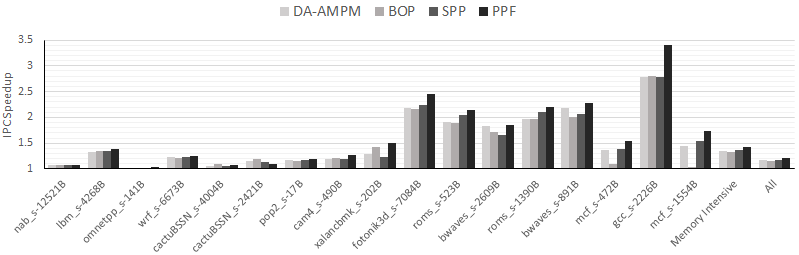
\includegraphics[width=\columnwidth]{SPEC2017}
\caption{SPEC CPU 2017 Single-Core IPC Speedup}
\label{Fig:SPEC2017_1core}
\end{figure}

\section{Results}
\label{Results}

This section discusses the results obtained from running PPF in terms of
prefetch cache coverage and speedup. For the SPEC CPU 2017 benchmarks, first
we present the results for single-threaded workloads then for multi-core
workloads.

\subsection{Single-core Results}
\label{Results-Single}

% djimenez: why is this figure described this way?  it's not OK to just
% highlight noticeable improvement. the benchmarks must be selected by some
% unbiased criteria, e.g. some minimum MPKI under LRU or some minimum speedup
% under a baseline prefetcher that isn't PPF.

Figure~\ref{Fig:SPEC2017_1core} shows the IPC speedup obtained by PPF,
compared to BOP, DA-AMPM and SPP.  In the figure we have depicted selected
traces where PPF shows a noticeable improvement or shows some degradation,
along with the geometric mean improvement on the memory intensive subset of
SPEC CPU 2017, and finally for the complete SPEC CPU 2017 benchmark.  All the
results have been normalized to the baseline of no prefetching.

% djimenez: you've inconsistently italicized and not italicized benchmark
% names. i'll help you out here; i like putting them in a typewriter font so
% i'll do that throughout this section. also, you've inconsistent put and not put
% the number of the benchmark. i'll fix that too.

PPF yields a geometric mean speedup of \textbf{42.8\%} over the baseline. 
This is equivalent to \textbf{7.8\%} over DA-AMPM, \textbf{9.7\%} over BOP 
and \textbf{6.92\%} over SPP.  Out of the 95 simpoints developed for SPEC 
CPU 2017, PPF nearly matches or outperforms most of the prefetchers on 91 
simpoints.  PPF fails to match the improvement offered by BOP only for 
{\tt 607.cactuBSSN\_s} and {\tt 654.roms\_s}.

At its peak, PPF manages a speedup of a factor of over \textbf{3.39x} on the
trace {\tt 602.gcc\_s-2226B}.  This also corresponds to speedup gain of
\textbf{60\%} over the next best prefetcher -- BOP.  In general, benchmarks
{\tt 603.bwaves\_s}, {\tt 605.mcf\_s}, {\tt 623. xalancbmk\_s} and {\tt
649.fotonik3d\_s} benefit the most from PPF, with the speedup over SPP ranging
from \textbf{10\% to 25\%}.

% djimenez: is this geometric mean? if so, say so.
% [EB] Resolved
On the full SPEC CPU 2017 suite, PPF improves the geometric mean IPC of 
the baseline by \textbf{20.9\%}, which is \textbf{3.44\%} better 
than the next best prefetcher -- SPP.
\newline

\begin{figure}[h]
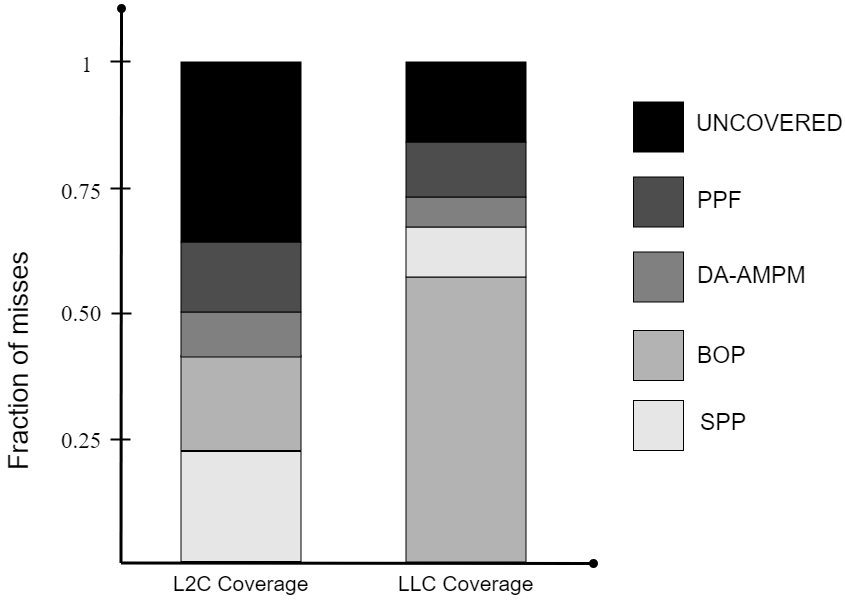
\includegraphics[width=\columnwidth]{Coverage}
\caption{Fraction of Cache Misses Covered}
\label{Fig:Coverage}
\end{figure}

% djimenez: this is a weird way to make a header for a section. use \paragraph or \subsection

\noindent \textbf{COVERAGE}
\newline
Prefetcher coverage is defined as the ratio of the number of misses avoided
through prefetching to the number of misses with no prefetching.

Figure~\ref{Fig:Coverage} shows the fraction of misses in the L2 and LLC
avoided by the various prefetchers.  PPF has the highest coverage of all the
prefetchers simulated. On the SPEC CPU 2017 benchmarks, PPF reduces misses by
\textbf{62.5\%} and \textbf{82.8\%} in the L2 and LLC respectively. For the
same benchmark, the next best prefetcher, DA-AMPM, covers \textbf{48.6\%} and
\textbf{72.8\%} of the misses respectively.

This superior coverage of PPF can be attributed to aggressive re-tuning of the
underlying SPP, enabled by the Perceptron Filter making sure the high coverage
does not lead to increased cache pollution.

\begin{figure*}[ht]
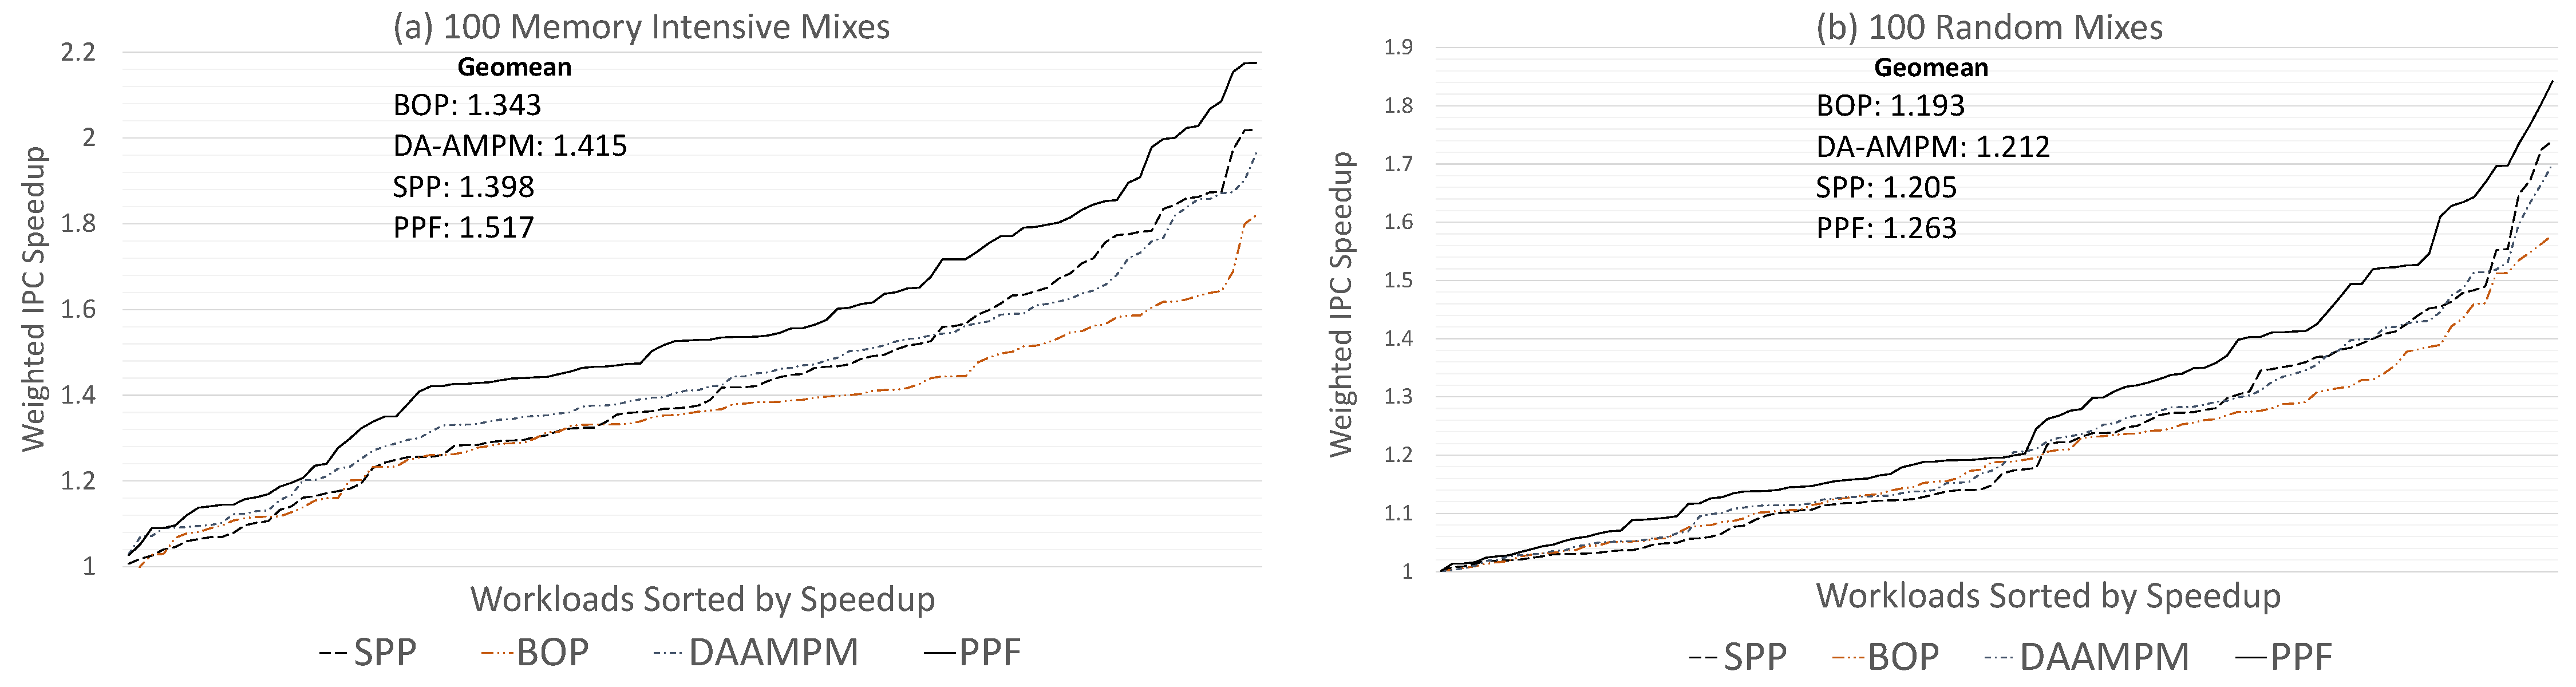
\includegraphics[width=\textwidth]{4Core_SPEC2017}
\caption{Normalized Speedup for 4-core SPEC CPU 2017 Workloads}
\label{Fig:4Core_SPEC2017}
\end{figure*}

\subsection{Multi-core Results}
\label{Results-Multi}
In this section, we demonstrate the improvement achieved by PPF for a mix of
multi-programmed workloads.
\newline

\noindent \textbf{4-CORE ENVIRONMENT}
\newline
Figure~\ref{Fig:4Core_SPEC2017}(a) shows a
comparison of speedups obtained on 4-core mixes of a memory intensive subset
SPEC CPU 2017.  We plot all 4 prefetchers, normalized to the baseline.  The
workloads have been sorted in increasing order of the speedup.  PPF offers a
speedup of \textbf{51.7\%} on these traces, and improvement of \textbf{11.9\%}
over the baseline SPP, \textbf{10.2\%} over the next DA-AMPM, and
\textbf{17.4\%} over BOP.

On a different set of fully random SPEC CPU 2017 4-core mixes, PPF provides an
IPC speedup of \textbf{26.2}\% over the baseline, which is an improvement of
\textbf{5.7}\% over SPP.
\newline

\begin{figure*}[ht]
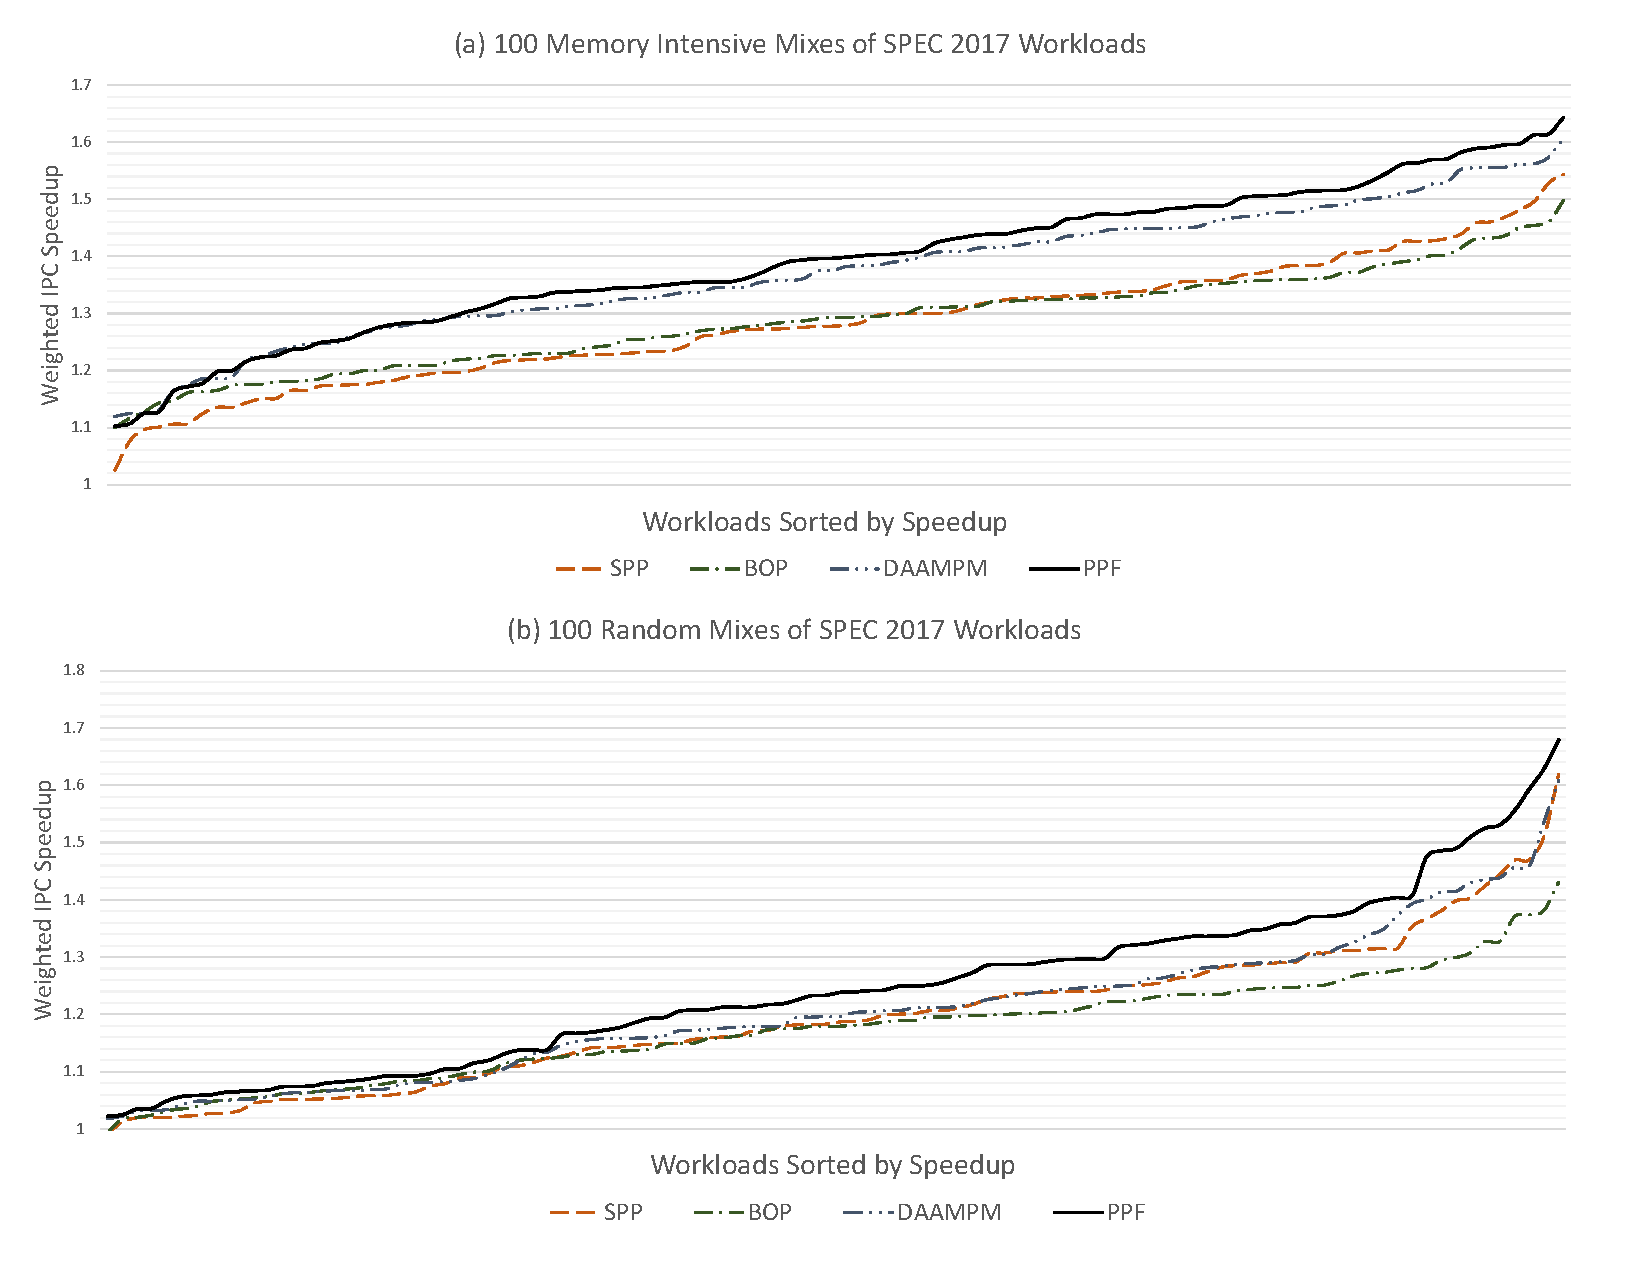
\includegraphics[width=\textwidth]{8Core_SPEC2017}
\caption{Normalized Speedup for 8-core SPEC CPU 2017 Workloads}
\label{Fig:8Core_SPEC2017}
\end{figure*}

\noindent \textbf{8-CORE ENVIRONMENT}
\newline
The sorted comparison of speedups on the memory
intensive 8-core mixes is shown in Figure~\ref{Fig:8Core_SPEC2017}.  PPF
improves baseline performance by \textbf{38.6\%}, an improvement of
\textbf{10.7\%} over SPP.  For a random set of SPEC CPU 2017 mixes, PPF
improves performance by \textbf{23.6\%} over the baseline, corresponding to
\textbf{4.8\%} over SPP.  This increased improvement achieved by PPF over the
base engine SPP in a multi-core environment is expected as PPF has a very
accurate filter, it eliminates useless prefetches before they can cause
pollution in the shared LLC.

BOP offers a better improvement than SPP for the memory intensive mixes. This
superiority can be attributed to BOP's inherent aggressive nature.  DA-AMPM is
also ahead of SPP in both the mixes. Interestingly, in all these cases, PPF
consistently outperforms the best performing prefetcher.

%[EB] How to justify only a small margin over DA-AMPM?

\begin{figure}[ht]
\begin{adjustwidth}{-1cm}{}
  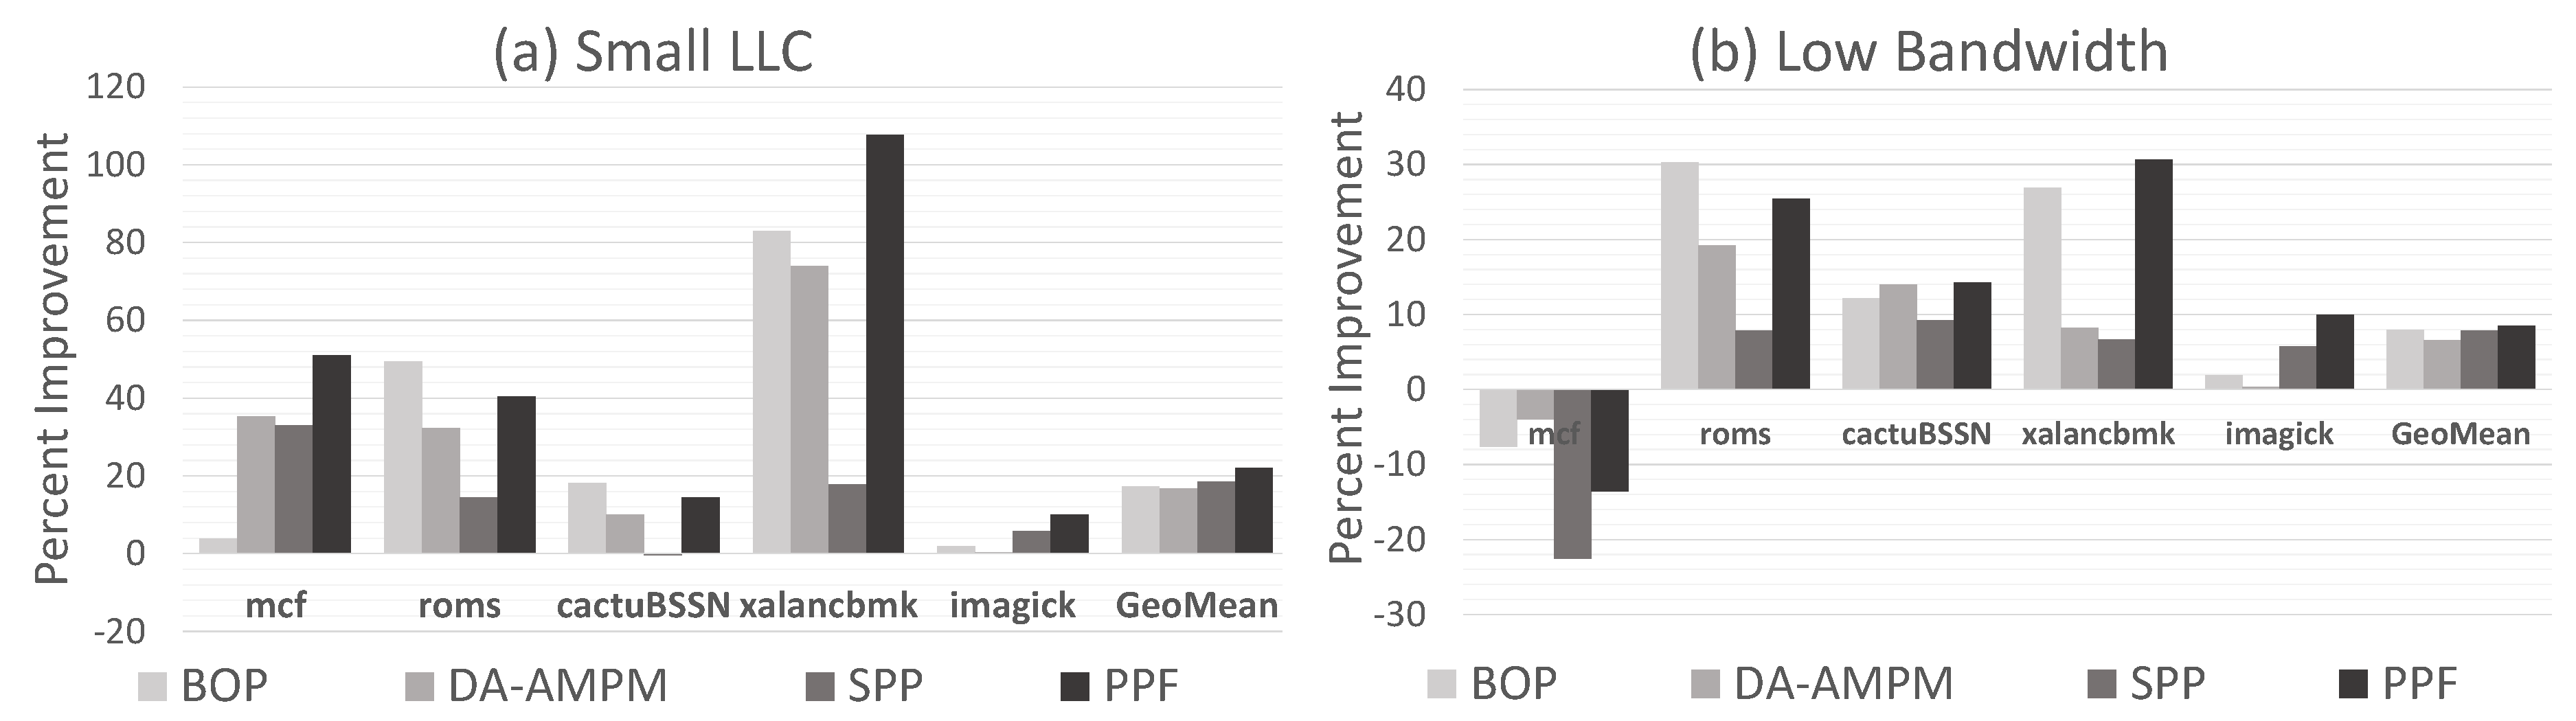
\includegraphics[width=1.2\columnwidth]{AddnConstr}
  \caption{IPC speedup for Small LLC and Low BW}
  \label{Fig:AddnConstr}
\end{adjustwidth}
\end{figure}

\subsection{Additional Memory Constraints}
\label{Results-AdditionalMem}

Figure~\ref{Fig:AddnConstr}(a) and (b) show the performance of PPF in a
reduced LLC and with low bandwidth constraints, respectively. For the sake of
brevity, we have only shown selected traces followed by the overall
performance on the complete benchmark.  Benchmark {\tt 605.mcf\_s} in low
bandwidth conditions is prefetch averse.  In general, any prefetcher yields a
negative speedup on that trace.  On {\tt 654.roms\_s} and {\tt
607.cactuBSSN\_s}, PPF is unable to match the performance achieved by the best
prefetcher. On the other hand, PPF outperforms all the other prefetchers on
{\tt 623.xalancbmk\_s} and {\tt 638.imagick\_s} benchmarks.  Overall, PPF gives
a better improvement under small LLC condition and matches the best
prefetcher, BOP, under low DRAM bandwidth conditions.

\begin{figure}[ht]
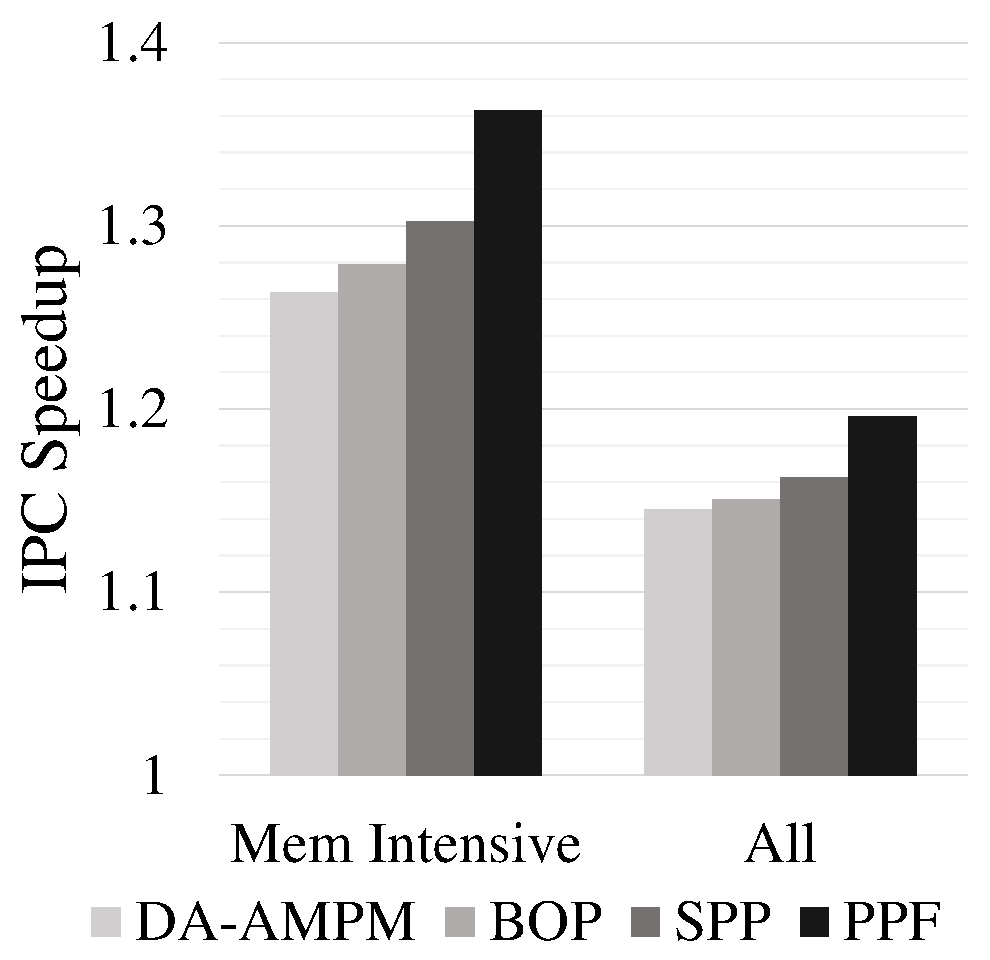
\includegraphics[width=\columnwidth]{SPEC2006}
\caption{SPEC CPU 2006 Single-Core IPC Speedup}
\label{Fig:SPEC2006_1core}
\end{figure}

\begin{figure}[ht]
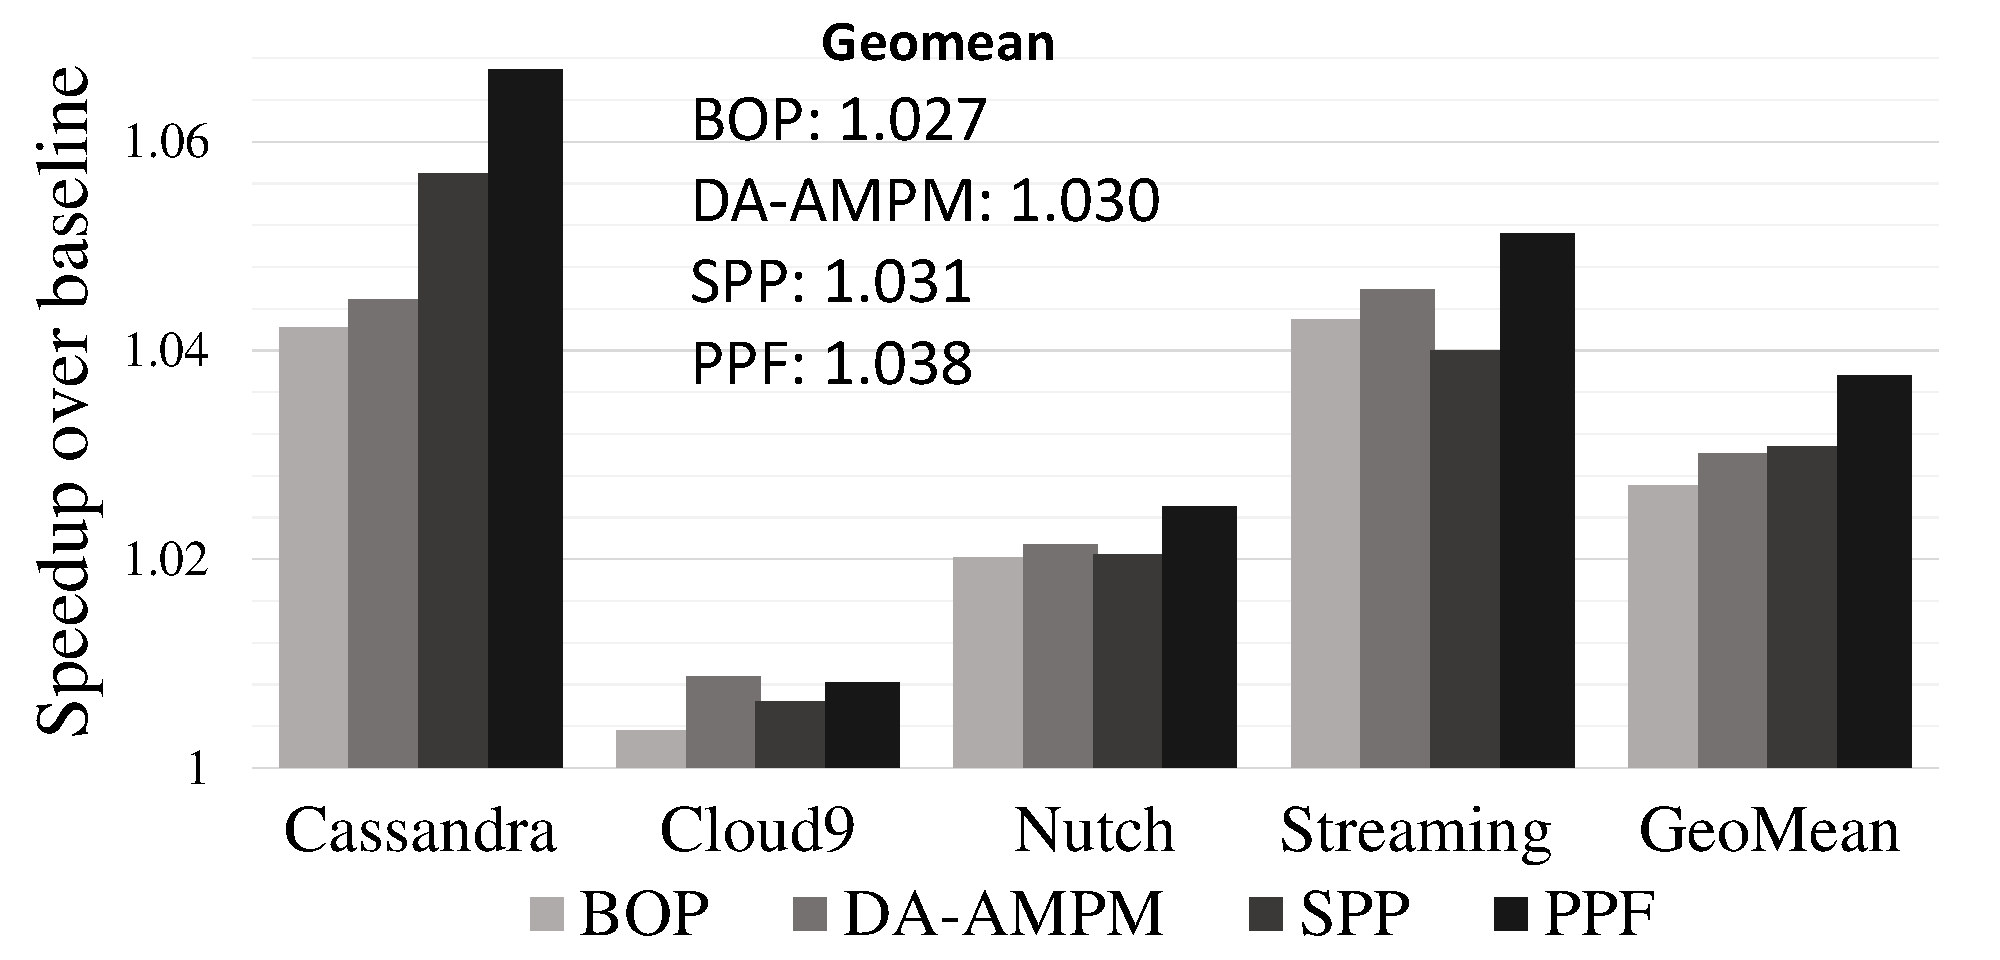
\includegraphics[width=\columnwidth,]{CloudSuite}
\caption{IPC Speedup for Multi-core CloudSuite Workloads}
\label{Fig:CloudSuite}
\end{figure}

\subsection{Cross Validation}
\label{Results-CrossVal}

% djimenez: cite cloudsuite here? do we have a reference?
% [EB]: Resolved. Cited "Clearing the clouds: A study of emerging 
%        scale-out workloads on modern hardware" in methodology

Here we demonstrate the robustness of PPF by testing it on different
benchmarks: SPEC CPU 2006 and CloudSuite.

% djimenez: is the improvement over BOP and DA-AMPM exactly the same 9.86%
% here? that's weird.
% [EB] Resolved. Increased precision of values. But yes, BOP / DA-AMPM 
% have really close numbers for SPEC 2006

Figure~\ref{Fig:SPEC2006_1core} shows the speed-up achieved by BOP, SPP and
PPF on traces from SPEC CPU 2006, along with the overall geometric mean over
the whole suite and over a memory-intensive subset.  PPF provides a speedup of
\textbf{46.1\%} over the baseline on the memory intensive subset of SPEC CPU
2006 benchmark, giving an improvement of \textbf{6.66\%} over SPP and
\textbf{9.88\%} over DA-AMPM and \textbf{9.82} over BOP.  On the whole of 
the SPEC CPU 2006 suite, the speedup is \textbf{22.4\%}, an improvement 
of \textbf{3.34\%} over SPP.

For 4-core memory intensive mixes, PPF improves the baseline by
\textbf{59.2\%}, \textbf{8.7\%} ahead of SPP. For 8-core memory intensive
mixes, the speedup over the baseline is \textbf{47.9\%}, \textbf{11.5\%} ahead
of SPP.

Figure~\ref{Fig:CloudSuite} shows the performance benefit comparison of all
the prefetch schemes on 4 different applications in the CloudSuite benchmark.
In general, these applications are prefetch agnostic. Even so, PPF manages a
\textbf{3.7\%} improvement over no prefetching, putting it ahead of the next
best prefetcher, SPP, which provides a 3.08\% speedup.

We developed PPF to yield good performance on the SPEC CPU 2017 benchmarks.
Nevertheless, the performance is consistently good on other benchmark suites.
We attribute this fact to the inherent adaptability of the perceptron model.
In general, perceptron weights are able to adjust in real-time so as to find
the best possible correlation between the output and the given set of
features.

\section{Related Work}
\label{related}

\subsection{Perceptrons in Cache Management}

In addition to branch prediction~\cite{PerceptronPredictor},
perceptron-based learning has been applied to the area of cache
management.  Teran \textit{et al.} propose using perceptrons to
predict cache line resuse, bypass, and replacement~\cite{Perc_Reuse}.
Perceptron Learning trains weights selected by hashes of multiple
features, including the PC of the memory access instruction, some
other recent PCs, and two different shifts of the tag of the
referenced block. These features are used to index into weight tables,
and the weights are then thresholded to generate a prediction. When a
block from one of a few sampled sets~\cite{sdbp} is reused or evicted,
the corresponding weights are decremented or incremented, according to
the perceptron learning rule. Multiperspective Reuse
Prediction~\cite{Multiperspective} improves on Perceptron Learning by
contributing many new features.

\subsection{Spatial Prefetchers}

Spatial prefetchers include such well-understood examples as the
next-line (or next-$n$-line) prefetcher, and the stream prefetcher,
and are distinguished by prefetching data without regard for the order
in which the data will be accessed.  In addition to these simpler
examples, Somogyi \textit{et al.}  propose Spatial Memory Streaming
(SMS)~\cite{SMS}.  SMS works by learning the spatial footprint of all
data used by a program within a region of memory around a given
missing load, and when the load that causes an new miss elsewhere, the
same spatial footprint is prefetched.  Ishii \textit{et al.} propose
the Access Map Pattern Matching prefetcher (AMPM)~\cite{AMPM}, which
creates a map of all accessed lines within a region of memory, and
then analyzes this map on every access to see if any fixed-stride
pattern can be identified and prefetched that is centered on the
current access. DRAM-Aware AMPM (DA-AMPM)~\cite{DA_AMPM} is a variant
of AMPM that delays some prefetches so they can be issued together
with others in the same DRAM row, increasing bandwidth utilization.
Pugsley \textit{et al.}  propose the Sandbox
Prefetcher~\cite{Sandbox}, which analyzes candidate fixed-offset
prefetchers in a sandboxed environment to determine which is most
suitable for the current program phase.  Michaud proposes the
Best-Offset Prefetcher~\cite{BOP}, which determines the optimal offset
to prefetch while considering memory latency and prefetch timeliness.

\subsection{Lookahead Prefetchers}

Unlike spatial prefetchers, lookahead prefetchers take program order
into account when they make predictions.  Shevgoor \textit{et al.}
propose the Variable Length Delta Prefetcher (VLDP)~\cite{VLDP}, which
correlates histories of deltas between cache line accesses within
memory pages with the next delta within that page. SPP~\cite{SPP} and
KPC's prefetching component~\cite{KPC} are more recent examples of
lookahead prefetchers. They try to predict not only what data will be
used in the future, but also the precise order in which the data will
be used, within a given page. Predictions made by lookahead
prefetchers can be fed back into their prediction mechanisms to
predict even further down a speculative path of memory acesses. These
prefetchers can also generalize their learned patterns from one page,
and use those patterns to make predictions in other pages.

\subsection{Managing Prefetched Data}

A low-accuracy aggressive prefetcher can significantly harm
performance.  To minimize interference from prefetching, Wu \textit{et
  al.} propose PACMan~\cite{pacman}, a prefetch-aware cache management
policy. PACMan dedicates some LLC sets to each of three competing
policies that treat demand and prefetch requests differently, using
the policy in the rest of the cache that shows the fewest
misses. Seshadri \textit{et al.} propose ICP~\cite{icp}, which demotes
a prefetch to the lowest reuse priority on a demand hit, based on the
observation that most prefetches are dead after their first hit. To
address prefetcher-caused cache pollution, it also uses a variation of
EAF~\cite{eaf} to track prefetching accuracy, and inserts only
accurate prefetches to the higher priority position in the LRU
stack. Jain \textit{et al.} propose Harmony~\cite{Harmony} to
accomodate prefetches in their MIN algorithm-inspired Hawkeye cache
management system. Ebrahimi \textit{et al.} introduce
HPAC~\cite{HPAC} which provides a coordinated control between 
multiple prefetchers present in a CMP by looking at the 
prefetcher-induced inter-core interferance.

\subsection{Machine Learning for Prefetching}

Peled \textit{et al.} introduce interesting ideas for on-line
Reinforcement Learning and dynamically scaling the magnitude of
feedback given to the baseline prefetcher~\cite{Semantics}. The
prefetcher relies on compiler support to receive features and build
the context.  Liao \textit{et al.}  focus on prefetching for data
center applications~\cite{Datacenter}.  They use offline machine
learning algorithms such as SVMs and logistic regression to do a
parametric search for an optimal prefetcher configuration. 
Hasheni \textit{et al.}~\cite{LSTM} categorize 
prefetching as a regression problem and use LSTM based Deep 
Learning approach.

\section{Conclusion}
\label{Conclusion}
In this paper, we introduced neural network based learning for data
prefetching in the form of PPF.  Perceptron acts an orthogonal
filter to the underlying prefetch engine.  PPF improves
performance by over XX\% over the baseline, which corresponds to YY\%
over the next best performing prefetcher.  
We believe that this is a robust and adaptable technique which can
be used to enhance any existing or upcoming prefetchers.

\end{spacing}

%%%%%%% -- PAPER CONTENT ENDS -- %%%%%%%%

%%%%%%%%% -- BIB STYLE AND FILE -- %%%%%%%%
\bibliographystyle{ieeetr}
\bibliography{ref}
%%%%%%%%%%%%%%%%%%%%%%%%%%%%%%%%%%%%

\end{document}
